\chapter{Prospects for differential \textsl{t}-channel measurements at 13~TeV}
\label{ch:prospects}

\intro{Prospects for a new differential single-top-quark cross section measurements in $t$~channel are discussed. The presented study is based on \gls{pp} collision data corresponding to 36~\invfb which were recored with the \gls{cms} experiment in 2016. A measurement of differential cross sections as a function of the top quark \pt, rapidity, and polarization angle is envisaged. Potential improvements include the training of a new \gls{bdt} discriminant and an extension of the fitting procedure for extracting the amount of single top quark events from data. Furthermore, the benefits for measuring differential cross sections at particle level compared to parton level are highlighted. For this, a technical study concerning the event selection at particle level for $t$-channel single-top-quark events is detailed which has also been published in Ref.~\cite{particleStudies}. The chapter is concluded by presenting results obtained with pseudo-data.}


%##############################################
\section{Setup}
%##############################################

Prospects for measuring differential single-top-quark cross sections as a function of the top quark \pt, rapidity, and the polarization angle at parton and particle level are studied in the following. The chosen analysis strategy is largely based on the one developed in the context of the first measurement of differential cross section of $t$-channel single-top-quark-production at 13~\TeV (Ch.~\ref{ch:diff13}). The setup of this study is outlined in the following.

The data statistics is increased by using \gls{pp} collision data corresponding to 36~\invfb which have been recored in 2016 with the \gls{cms} detector at a \acrlong{cm} energy of 13~\TeV. Events containing an isolated muon candidate and two or three jets are selected using mostly the criteria detailed in Sec.~\ref{sec:diff13-selection} with a few exceptions as highlighted below. Due to the higher instantaneous luminosity in the 2016 data-taking period compared to 2015 which peaked at $15.3~\mathrm{Hz}/\mathrm{nb}$~\cite{lumipublic}, the threshold of the employed single muon trigger has been raised to $24~\GeV$. Consequently, muon candidates with a higher threshold of $\pt>26~\GeV$ are required offline as well. All other muon selection criteria are kept the same. The analysis of events containing single electrons and two or three jets is also envisaged for a potential update of the differential cross section measurement. Corresponding data events are recorded with an electron trigger that requires an electron candidate with a transverse momentum of at least $32~\GeV$ within $|\eta|<2.1$. Offline, events must contain a corresponding electron candidate with $\pt>35~\GeV$ within $|\eta|<2.1$. In addition, an electron candidate has to fulfill tight identification criteria which have been specifically designed to select mostly genuine electrons~\cite{CMS-DP-2017-004}.

For b-tagging a new algorithm, the so-called \gls{cmva}-tagger (combined MVA)~\cite{CMS-PAS-BTV-15-001} is employed which includes amongst others the output of the previously used \gls{csv} algorithm in its training. Both algorithms have a mistagging rate of only 0.1\% for light-flavored jets originating from u,d,s quarks and gluons at their corresponding tight working points. An efficiency of about 55\% is obtained for tagging true b~jets with the \gls{cmva}-tagger which is approximately 10\% higher than the b-tagging efficiency of the \gls{csv} algorithm. 

The remainder of the event selection is kept identical to Sec.~\ref{sec:diff13-selection} which includes the veto of events containing additional leptons, the jet clustering, and the categorization of events into signal and control regions based on the number of selected jets and b-tags.

The following samples of simulated events are used for this study. A sample of single-top-quark $t$-channel events has been generated with the \POWHEG generator interfaced with \PYTHIA{}8 and \MADSPIN. The \POWHEG generator interfaced with \PYTHIA{}8 is also used to generated events of tW single-top-quark and \ttbar production. Samples of \wjets and \zjets production are generated with the \MGAMC generator interfaced with \PYTHIA{}8. Exclusive \wjets samples with zero, one, or two extra jets are generated and merged with the \gls{fxfx} procedure~\cite{Frederix:2012ps}. The cross sections for normalizing these samples are identical to the ones used in Ch.~\ref{ch:diff13} and can be found in Tab.~\ref{tab:diff13-theo-xsecs} with the exception of the exclusive \wjets cross sections which are listed in Tab.~\ref{tab:prospects-theo-xsecs}.

\mytable{\label{tab:prospects-theo-xsecs}Theoretical \gls{sm} cross sections used to normalize the exclusive \wjets samples.}{
\begin{tabular}{@{}l  r c l@{}}
\toprule
$\mathrm{W}\to\ell\nu\mathrm{\,\mbox{+}\,0~jets}$ & $49\,670~\pb$ && \gls{nlo} \hfill (reported by \MGAMC) \\
$\mathrm{W}\to\ell\nu\mathrm{\,\mbox{+}\,1~jet}$ & $8\,264~\pb$ && \gls{nlo} \hfill (reported by \MGAMC) \\
$\mathrm{W}\to\ell\nu\mathrm{\,\mbox{+}\,2~jets}$ & $2\,544~\pb$ && \gls{nlo} \hfill (reported by \MGAMC) \\
\bottomrule
\end{tabular}
}


The contamination by multijet events are estimated in muon and electron channel through templates extracted from data in a sideband region. In the muon channel, the sideband region is defined by inverting the relative isolation as $\muiso>20\%$. In the electron channel the isolation requirement is part of the used tight identification criteria. A sideband region is defined in the electron channel by inverting corresponding loose identification criteria. The resulting description of data by the multijet templates is validated in the 2j0t control region. In Fig.~\ref{fig:pospects-met-wjets} the \met distribution and the distribution of the difference in $\phi$ angles between the lepton and the transverse momentum vector are presented for both channels after scaling the templates to the result of a \gls{ml} fit as detailed in Sec.~\ref{sec:prospects-fit}. The \met distributions display a good agreement between data and predictions in both channels. A good description of data by the multijet template is also achieved for the $\Delta\phi(\mu,\met)$ distribution in the muon channel. However, a slight mismodeling is observed in the electron channel (Fig.~\ref{fig:pospects-met-wjets-ele-phi}) in the $\Delta\phi(\mu,\met)$ distribution for which some further finetuning of the sideband region is planned which may improve the extracted multijet shape.

Distributions of the reconstructed top quark mass in the 2j1t signal and 3j1t/3j2t \ttbar control regions are presented in Fig.~\ref{fig:pospects-topmass} for muon and electron channel. A fair modeling is observed for both channels although a slight slope can be seen in the data-to-\gls{mc} ratio for the electron channel which may however not be significant when evaluating the impact by systematic uncertainties. The additional b-tag requirement reduces the contribution by multijet events in both channels to a comparable fraction as opposed to the 2j0t control region (Fig.~\ref{fig:pospects-met-wjets}) where the electron channel appears to be contaminated by more than twice as many multijet events as the muon channel. 


\myfigure{\label{fig:pospects-met-wjets} Distributions of (top row)~the transverse missing energy and (bottom row)~the difference in $\phi$ angle between the lepton and the missing transverse energy in the 2j0t control region for (a)~electron and (b)~muon events.}{
\subfloat[]{\adjincludegraphics[height=4.8cm,trim={0 0 {0.16\width} 0},clip]{figures/prospects/plots/2j0t/electron_2j0t_met_qcdnone_nol.pdf}}
\subfloat[]{\adjincludegraphics[height=4.8cm,trim={0 0 {0.\width} 0},clip]{figures/prospects/plots/2j0t/muon_2j0t_met_qcdnone.pdf}}\\
\subfloat[\label{fig:pospects-met-wjets-ele-phi}]{\adjincludegraphics[height=4.8cm,trim={0 0 {0.16\width} 0},clip]{figures/prospects/plots/2j0t/electron_2j0t_lepton_met_deltaPhi_qcdnone_nol.pdf}}
\subfloat[]{\adjincludegraphics[height=4.8cm,trim={0 0 {0.\width} 0},clip]{figures/prospects/plots/2j0t/muon_2j0t_lepton_met_deltaPhi_qcdnone.pdf}}
}

\myfigure[p]{\label{fig:pospects-topmass} Distributions of the reconstructed top quark mass for (left column)~electron and (right column)~muon channel: (top row)~signal region; (middle and bottom row)~\ttbar control region.}{
\subfloat[]{\adjincludegraphics[height=4.8cm,trim={0 0 {0.16\width} 0},clip]{figures/prospects/plots/2j1t/electron_2j1t_top_mass_qcdnone_nol.pdf}}
\subfloat[]{\adjincludegraphics[height=4.8cm,trim={0 0 {0.\width} 0},clip]{figures/prospects/plots/2j1t/muon_2j1t_top_mass_qcdnone.pdf}}\\
\subfloat[]{\adjincludegraphics[height=4.8cm,trim={0 0 {0.16\width} 0},clip]{figures/prospects/plots/3j1t/electron_3j1t_top_mass_qcdnone_nol.pdf}}
\subfloat[]{\adjincludegraphics[height=4.8cm,trim={0 0 {0.\width} 0},clip]{figures/prospects/plots/3j1t/muon_3j1t_top_mass_qcdnone.pdf}}\\
\subfloat[]{\adjincludegraphics[height=4.8cm,trim={0 0 {0.16\width} 0},clip]{figures/prospects/plots/3j2t/electron_3j2t_top_mass_qcdnone_nol.pdf}}
\subfloat[]{\adjincludegraphics[height=4.8cm,trim={0 0 {0.\width} 0},clip]{figures/prospects/plots/3j2t/muon_3j2t_top_mass_qcdnone.pdf}}
}
 
\clearpage

%##############################################
\section{New BDT discriminant}
%##############################################

One shortcoming in the previous measurements within this thesis was the lack of a \wjets control region enriched by heavy-flavored jets. Such a region would allow to validate the \wjets modeling in greater detail. Furthermore, including such a region in the \gls{ml} fit may help to reduce the correlations between the estimated signal and background yields further. An approach to achieve this is to train an additional \gls{bdt}, referenced \bdttt in the following, for separating \wjets from \ttbar events. Even observables which are correlated to the unfolding variables can be used safely in its training if the resulting discriminant is not used in a signal-enriched region for the measurement. The following observables have been chosen as input for the training:

\begin{itemize}
\item the invariant mass of the reconstructed top quark candidate;
\item the missing transverse energy, \met;
\item the transverse momentum of the dijet system, $(\vec{p}_\mathrm{b}+\vec{p}_{\jprime})_\mathrm{T}$;
\item the event shape C (introduced in Sec.~\ref{sec:diff13-bdt});
\item the $\Delta R$ distance between the two jets;
\item the $\Delta R$ distance between the b-tagged jet and the lepton;
\item the invariant mass of the \acrlong{cm} system; $\sqrt{\hat{s}}=|p_\mathrm{top}+p_{\jprime}|$;
\item the W~boson helicity angle, $\cos\theta_\mathrm{W}^\star$, defined between the top quark and lepton momentum in the W~boson rest frame (see Sec.~\ref{sec:theory-top-quark-decay} for details);
\end{itemize}

The distribution of the W~boson helicity angle is shown in Fig.~\ref{fig:prospects-cosWhel}. A good agreement between data and prediction is observed in the muon and electron channel. The angle is reconstructed under the $t$-channel single-top-quark hypothesis but it might often overlap here with the proper angle for \ttbar events in cases where the selected b-tagged jet and lepton originate from the decay of the same top quark in \ttbar events. For \wjets events on the other hand this angle has no physical meaning. Hence its distribution provides separation power for discriminating \ttbar against \wjets events in the \gls{bdt} training.

\myfigure{\label{fig:prospects-cosWhel} Distributions of the W~boson helicity angle in 2j1t (a)~electron and (b)~muon channel.}{
\subfloat[]{\adjincludegraphics[height=4.8cm,trim={0 0 {0.16\width} 0},clip]{figures/prospects/plots/2j1t/electron_2j1t_cosTheta_wH_qcdnone_nol.pdf}}
\subfloat[]{\adjincludegraphics[height=4.8cm,trim={0 0 {0.\width} 0},clip]{figures/prospects/plots/2j1t/muon_2j1t_cosTheta_wH_qcdnone.pdf}}
}


The resulting \bdttt discriminant is presented in Fig.~\ref{fig:prospects-bdt-tt} in a signal-depleted region. A fair description of data by the prediction is observed. An \gls{auc} of about 25\% is obtained in both channels for separating \ttbar from \wjets events. Although this new discriminant does yield a region dominated by W+heavy flavored jets, its distribution can be exploited for improving the \gls{ml} fit result.

\myfigure{\label{fig:prospects-bdt-tt} Distributions of the \bdttt discriminant, trained for separating \ttbar from \wjets events, in 2j1t (a)~electron and (b)~muon channel.}{
\subfloat[]{\adjincludegraphics[height=4.8cm,trim={0 0 {0.16\width} 0},clip]{figures/prospects/plots/2j1t/electron_2j1t_bdt_ttw_boost04_CR_nol.pdf}}
\subfloat[]{\adjincludegraphics[height=4.8cm,trim={0 0 {0.\width} 0},clip]{figures/prospects/plots/2j1t/muon_2j1t_bdt_ttw_boost04_CR.pdf}}
}

The signal-depleted region is defined by selecting events with $\bdttch<0$ using the discriminant of a second \gls{bdt} trained for separating signal from \wjets and \ttbar events. This second \gls{bdt}, \bdttch, that has been trained similar to the one used in Sec.~\ref{sec:diff13-bdt}. The distribution of its discriminant is shown in Fig.~\ref{fig:prospects-bdt-tch} where however data in the signal-enriched region ($\bdttch>0$) has been blinded since the strategy of the envisaged measurement is under development. It will be unblinded when the strategy has been finalized.

\myfigure{\label{fig:prospects-bdt-tch} Distributions of the \bdttch discriminant, trained for separating signal from \ttbar and \wjets events, in 2j1t (a)~electron and (b)~muon channel. Data has been blinded in the signal-enriched region $\bdttch>0$.}{
\subfloat[]{\adjincludegraphics[height=4.8cm,trim={0 0 {0.16\width} 0},clip]{figures/prospects/plots/2j1t/electron_2j1t_bdt_tch_boost04_qcdnone_blind_nol.pdf}}
\subfloat[]{\adjincludegraphics[height=4.8cm,trim={0 0 {0.\width} 0},clip]{figures/prospects/plots/2j1t/muon_2j1t_bdt_tch_boost04_qcdnone_blind.pdf}}
}

%##############################################
\section{Signal extraction}
%##############################################
\label{sec:prospects-fit}

The amount of signal is estimated by performing a template-based \gls{ml} fit to data. The distributions of the transverse W~boson mass and the two \gls{bdt} discriminants are used to construct a compound template as follows. The \mtw distribution as shown in Fig.~\ref{fig:pospects-fit-templ-mtw} is used for events with $\mtw<50~\GeV$ which provides sensitivity to the multijet event yield. The remaining events are split in two additional regions based on the \bdttch discriminant. For event with $\bdttch<0$ the \bdttt distribution is fitted as presented in Fig.~\ref{fig:pospects-fit-templ-bdttt} which is sensitive to the \wjets and \ttbar yields while the amount of signal events is negligible in this region as shown in Fig.~\ref{fig:prospects-bdt-tt}. Lastly, the \bdttch distribution is used for the remainder of events that fall in the region defined by $\bdttch>0$ and $\mtw>50~\GeV$. This region provides sensitivity to the amount of signal events which can be seen in Figs.~\ref{fig:pospects-fit-templ-bdttch} and~\ref{fig:prospects-bdt-tch}.

\myfigure{\label{fig:pospects-fit-templ}Shape comparison of the fit components in 2j0t: (a) transverse W~boson mass; (b)~\bdttt discriminant trained to separate \ttbar from \wjets events; (c)~\bdttch discriminant trained to separate signal from \ttbar and \wjets events.}{
\subfloat[\label{fig:pospects-fit-templ-mtw}]{\adjincludegraphics[height=4.8cm,trim={0 0 {0.16\width} 0},clip]{figures/prospects/fit/comp_2j1t_mtw_mtwinv_nol.pdf}}
\subfloat[\label{fig:pospects-fit-templ-bdttt}]{\adjincludegraphics[height=4.8cm,trim={0 0 {0.\width} 0},clip]{figures/prospects/fit/comp_2j1t_bdt_ttw_boost04_bdtinv.pdf}}\\
\subfloat[\label{fig:pospects-fit-templ-bdttch}]{\adjincludegraphics[height=4.8cm,trim={0 0 {0.\width} 0},clip]{figures/prospects/fit/comp_2j1t_bdt_tch_boost04_bdt.pdf}}
}

In addition to the 2j1t region, the two \ttbar control region (3j1t,3j2t) are fitted simultaneously as well. Similar to the strategy described in Sec.~\ref{sec:diff13-fit} multiple \gls{ml} fits are performed to estimated the amount of signal events as a function of the top quark \pt, rapidity, and the polarization angle.

 

%##############################################
\section{Particle level selection}
%##############################################
\label{sec:prospects-fiducial-studies}

Measuring differential cross sections at particle level has various benefits compared to the parton level as discussed in Sec.~\ref{sec:technique-levels}. In this section a technical study about the reconstruction and selection of analysis objects at particle level for $t$-channel single-top-quark production is described which has also been published in Ref.~\cite{particleStudies}.


The distribution of the transverse momentum of the muon at reconstruction level is presented in Fig.~\ref{fig:prospects-particle-muon} after selecting events with one muon without any requirements on the number of jets. At particle level events are selected containing a dressed muon candidate with a transverse momentum of at least $26~\GeV$ within $|\eta|<2.4$ which follows the kinematic selection at reconstruction level. At parton level, events are only required to posses a muon from a top quark decay without applying any kinematic constraints. In the top panel of Fig.~\ref{fig:prospects-particle-muon} the overlap of common events selected at parton or particle level which are also selected at reconstruction level is shown. The bottom panel displays the corresponding acceptance of selecting parton/particle-level events at reconstruction level. A large overlap~($>99\%$) between all three distributions is observed which demonstrates that nearly all events that are selected at reconstruction level can also be found at the particle and parton level. It should be noted that if muons from intermediate prompt tau leptons would be excluded from the utilized dressed lepton definition this overlap reduces to about 94\% instead. One can observe that the acceptance increases towards higher muon momenta which is a consequence of the muon isolation and identification requirements at reconstruction level that become less stringent. 

\myfigure{\label{fig:prospects-particle-muon}Distributions of the transverse muon momentum after requiring events with one muon at reconstruction, particle, or parton level. No requirement on the number of jets is made. Top panel: common events selected at reconstruction level; bottom panel: acceptance of reconstruction level selection. The figures are taken from Ref.~\cite{particleStudies}.}{
\subfloat[\label{fig:prospects-particle-level-muonpt}]{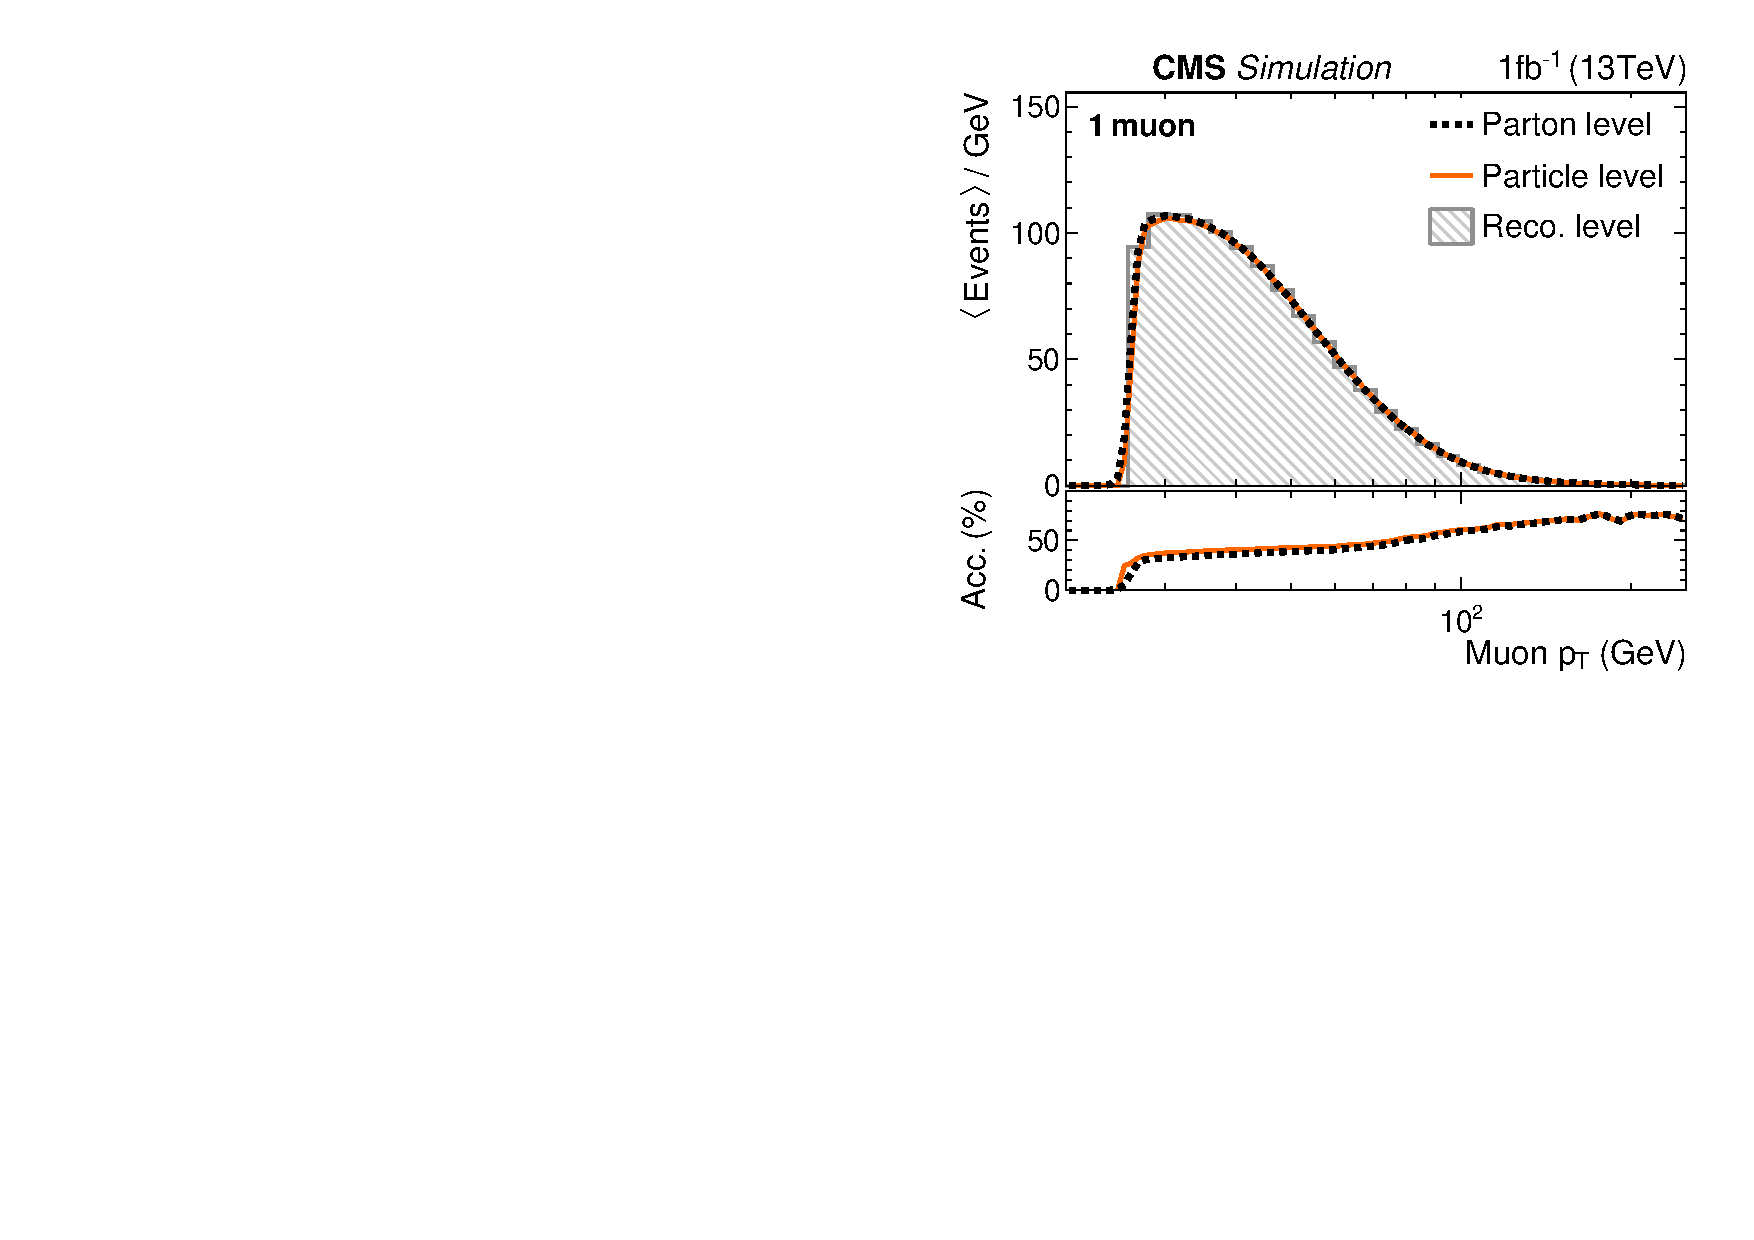
\includegraphics[width=0.48\textwidth]{figures/prospects/fiducial/muon_particle_logpt.pdf}}\hspace{0.03\textwidth}
\subfloat[\label{fig:prospects-particle-level-muoneta}]{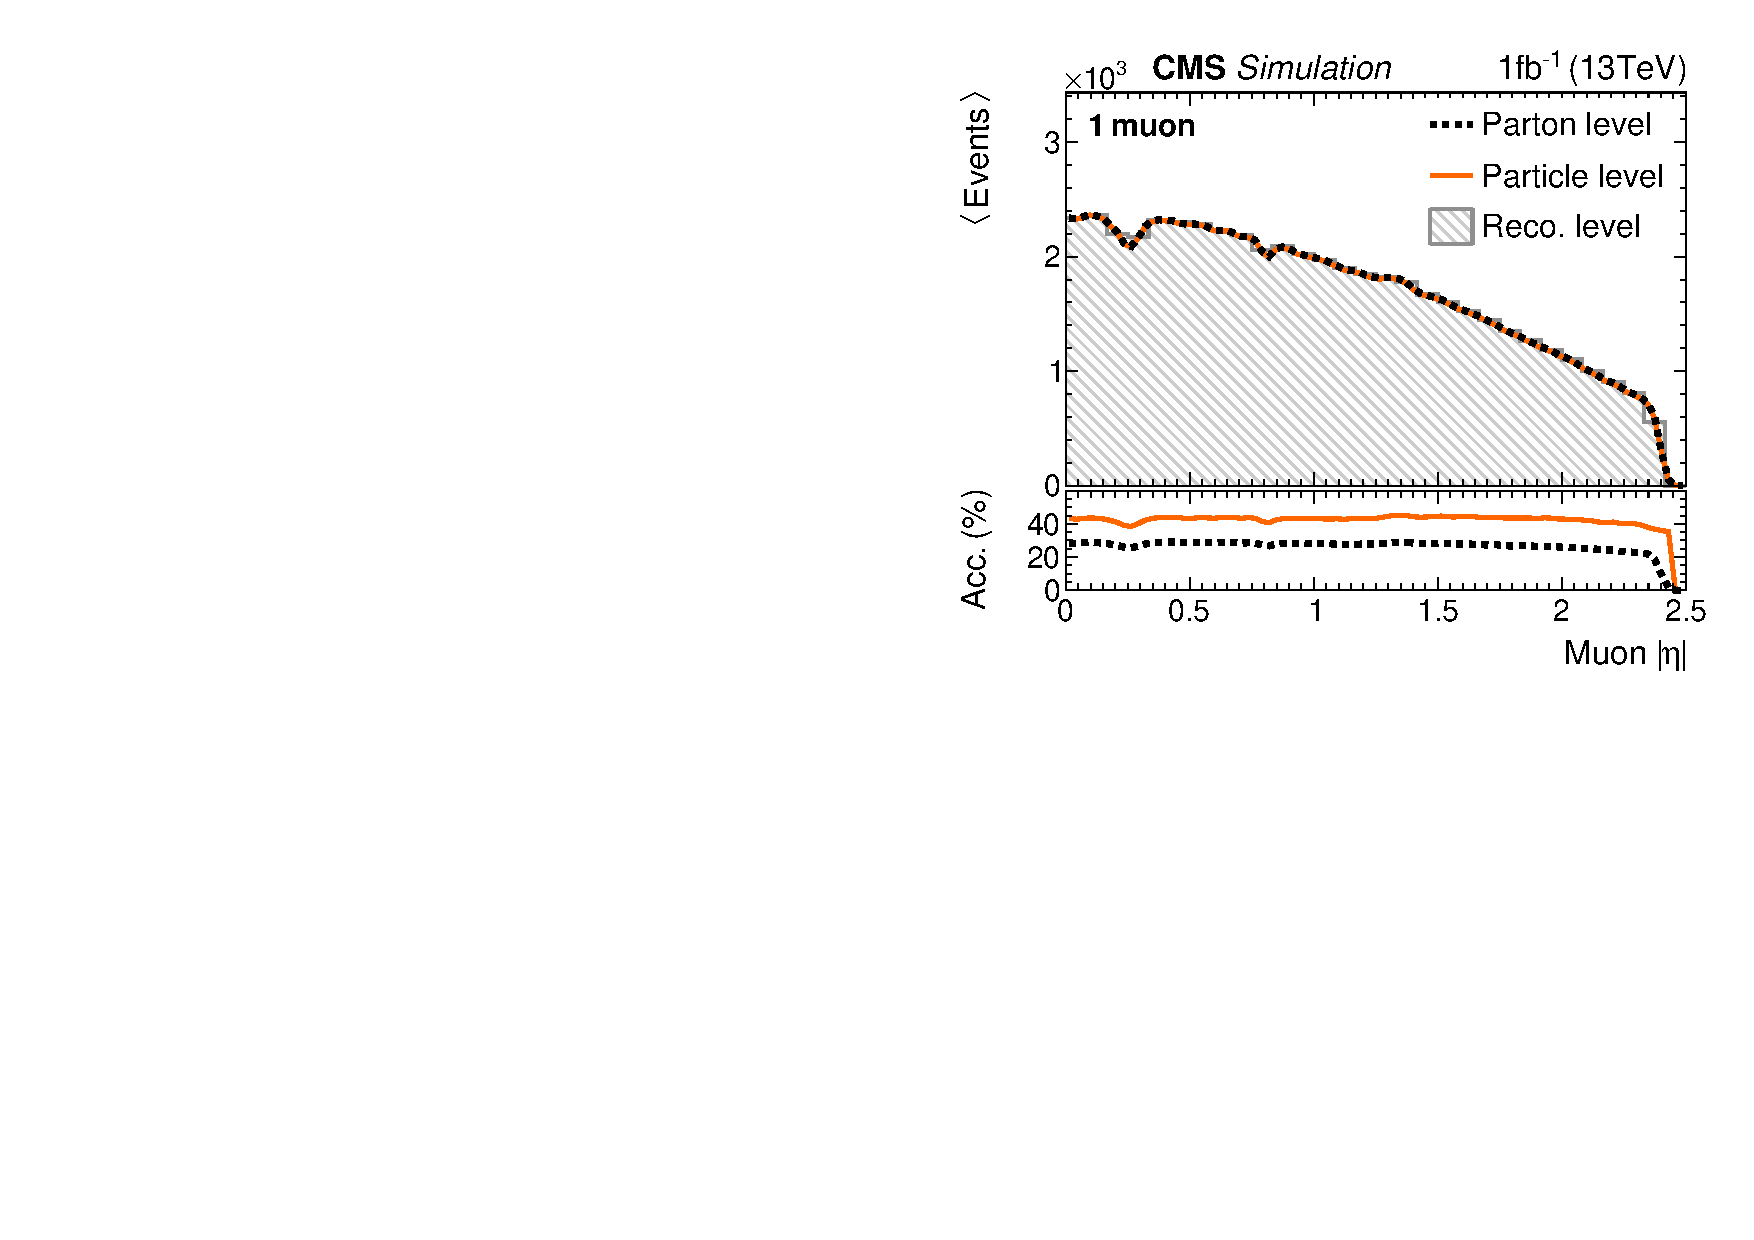
\includegraphics[width=0.48\textwidth]{figures/prospects/fiducial/muon_particle_abseta.pdf}}
}

Jets with a transverse momentum of at least $40~\GeV$ within $|\eta|<4.7$ are selected at particle level which have been clustered from stable particles excluding neutrinos and the prompt leptons and photons used in the dressed lepton reconstruction. The amount of selected jets for events passing the muon selection step is shown in Fig.~\ref{fig:prospects-particle-njets}. At reconstruction level, events with at least two jets are shown while no requirement on the number of jets is made at particle level. When selecting events with exactly two jets at reconstruction and particle level simultaneously, the amount of events at reconstruction level overlapping with the selected events at particle level reduces to about 80\%. The remaining 20\% of events at reconstruction level have not been selected at particle level due to the broad jet energy resolution leading to a migration of events into either the first or the third jet bin at particle level.

The number of b-tagged jets is shown in Fig.~\ref{fig:prospects-particle-njets} after requiring exactly two jets in the event at particle and reconstruction level. 
At the particle level, the number of b-tagged jets is counted with the ghost-B-hadron method~\cite{Cacciari:2008gn}. The distribution reveals that a certain fraction of events has two ghost-b-tagged jets despite events with only one b-tagged jet are selected at reconstruction level. This is a consequence of the ghost-B-hadron method which has a relatively high efficiency for tagging true b~jets compared to the employed \gls{cmva} algorithm at reconstruction level. Selecting events with only one b-tagged jet at the particle level results in a degradation in the overlap to about 70\% which is considered a non-negligible loss. Thus, in this study no requirement on the number of b-tagged jets is imposed. This simplification leads to a jet assignment problem for the pseudo-top quark definition which is solved by associating the jet that yields an invariant pseudo-top quark mass (together with the muon and neutrino candidate) which is closest to $172.5~\mathrm{GeV}$.

\myfigure{\label{fig:prospects-particle-jets}Distributions of the number of jets (left) for events with at least two selected jets at reconstruction level and number of b-tagged jets (right) for events with two selected jets at reconstruction and particle level. Top panels: common events selected at reconstruction level; bottom panels: acceptance of reconstruction level selection. The figures are taken from Ref.~\cite{particleStudies}.}{
\subfloat[\label{fig:prospects-particle-njets}]{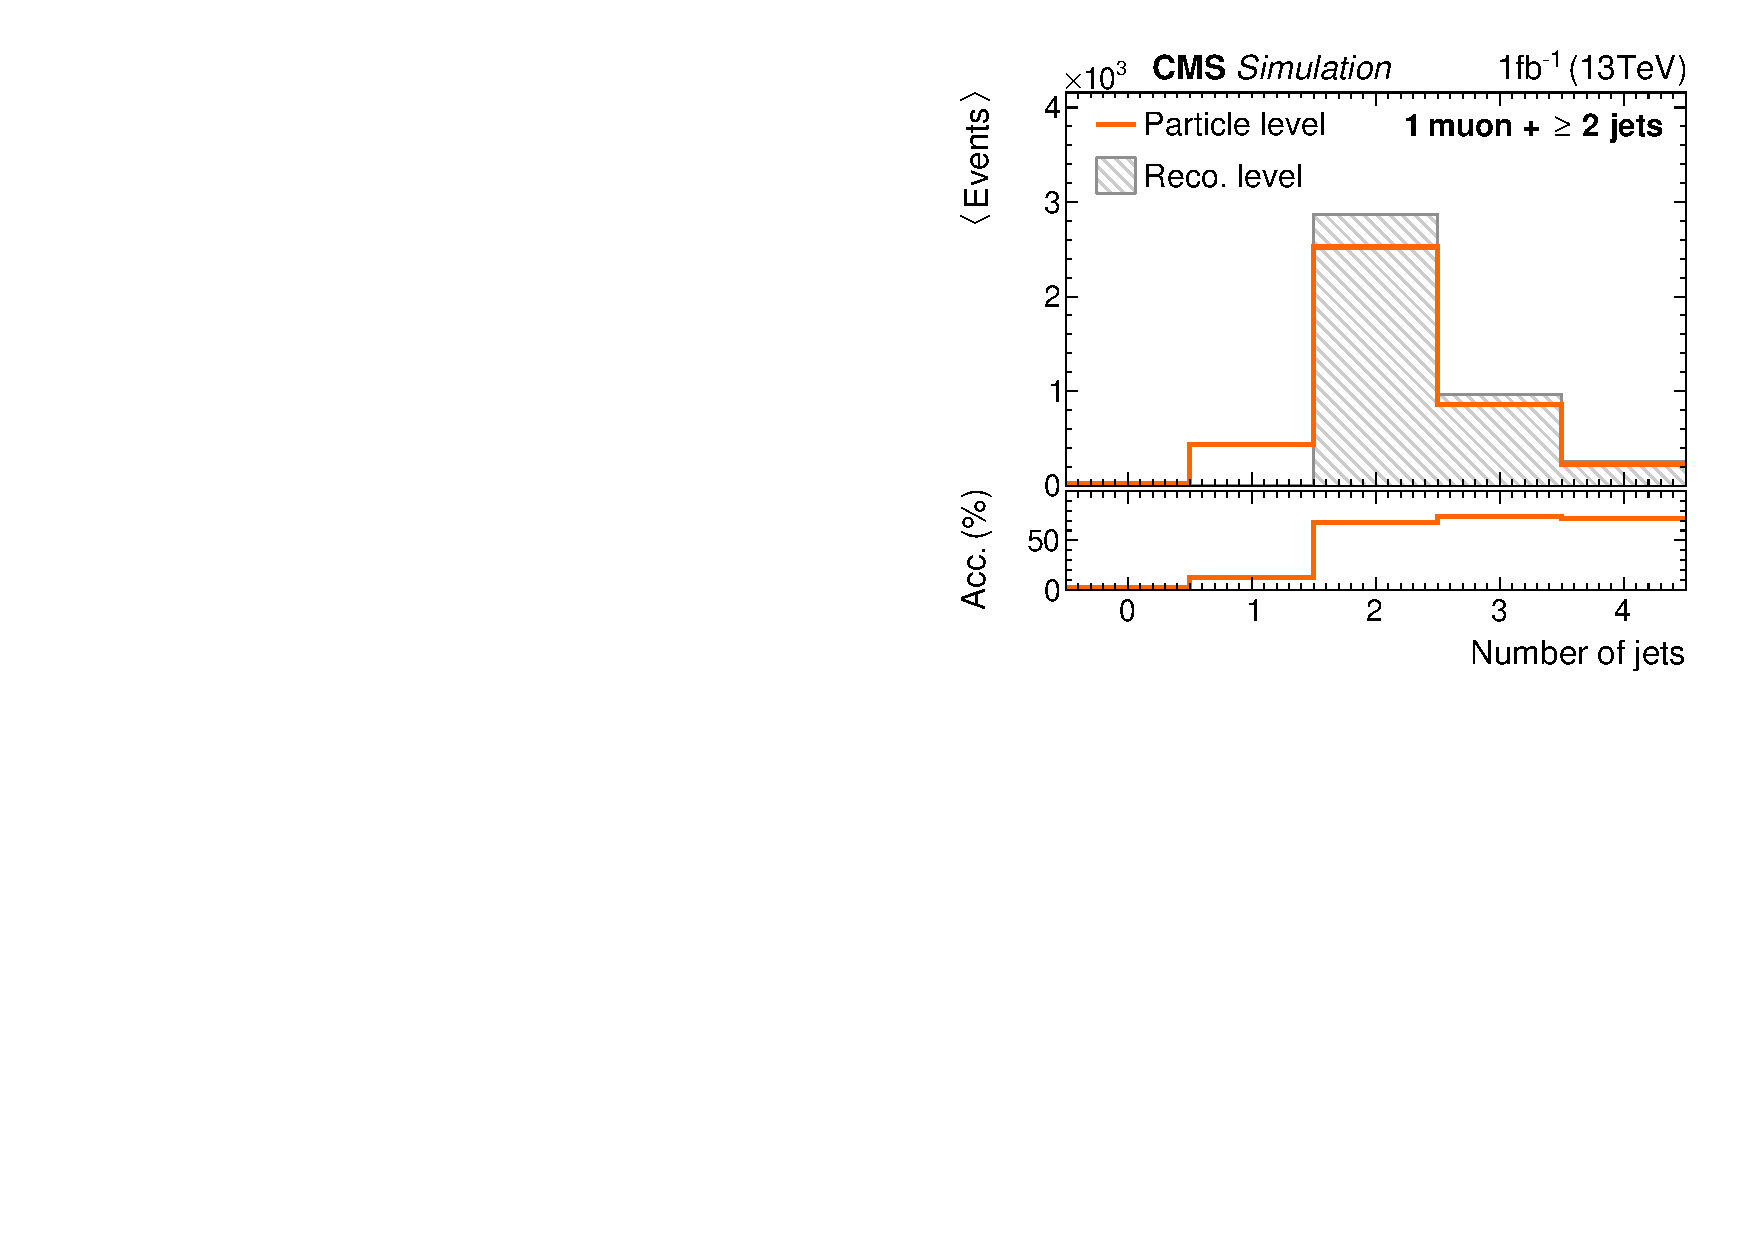
\includegraphics[width=0.48\textwidth]{figures/prospects/fiducial/njet_particle.pdf}}\hspace{0.03\textwidth}
\subfloat[\label{fig:prospects-particle-nbjets}]{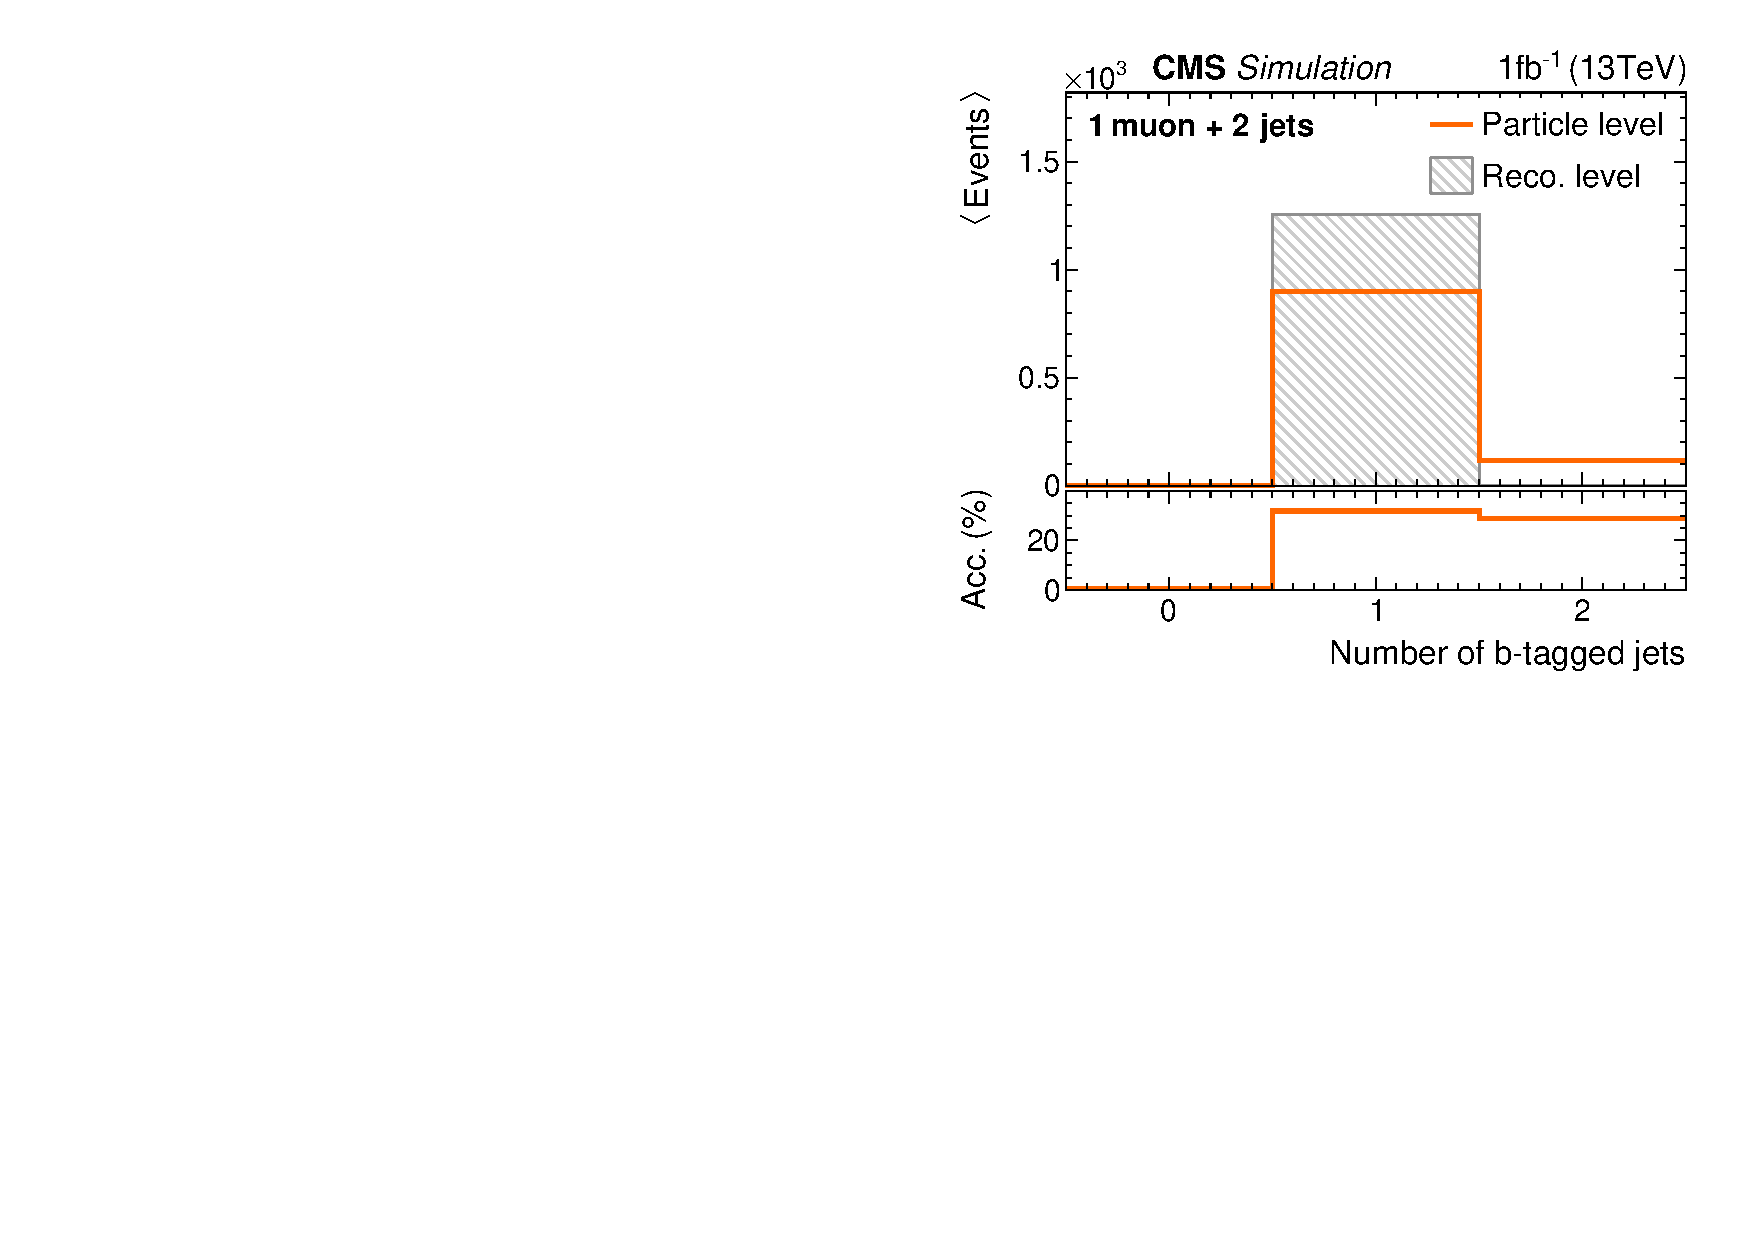
\includegraphics[width=0.48\textwidth]{figures/prospects/fiducial/nbjet_particle.pdf}}
}

The distributions of the \pt and pseudorapidity of the (untagged) jet originating from the spectator quark are shown in Fig.~\ref{fig:prospects-particle-ljet}. 
At particle level, it is the jet which is not associated to the pseudo-top quark decay by the invariant mass criterion. 
The observed turn-on in the \pt distribution confirms that the drop in the overlap between reconstruction and particle level from $>99\%$ after the muon selection step down to 80\% after requiring also two jets in the events is attributed to the jet energy resolution. The overlap can be increased by lowering the transverse momentum threshold of jets at particle level which has however not been studied further in the context of this study.

\myfigure{\label{fig:prospects-particle-ljet}Distributions of the spectator jet: (left) transverse momentum; (right) absolute value of the pseudorapidity. Top panels: common events selected at reconstruction level; bottom panels: acceptance of reconstruction level selection. The figures are taken from Ref.~\cite{particleStudies}.}{
\subfloat[]{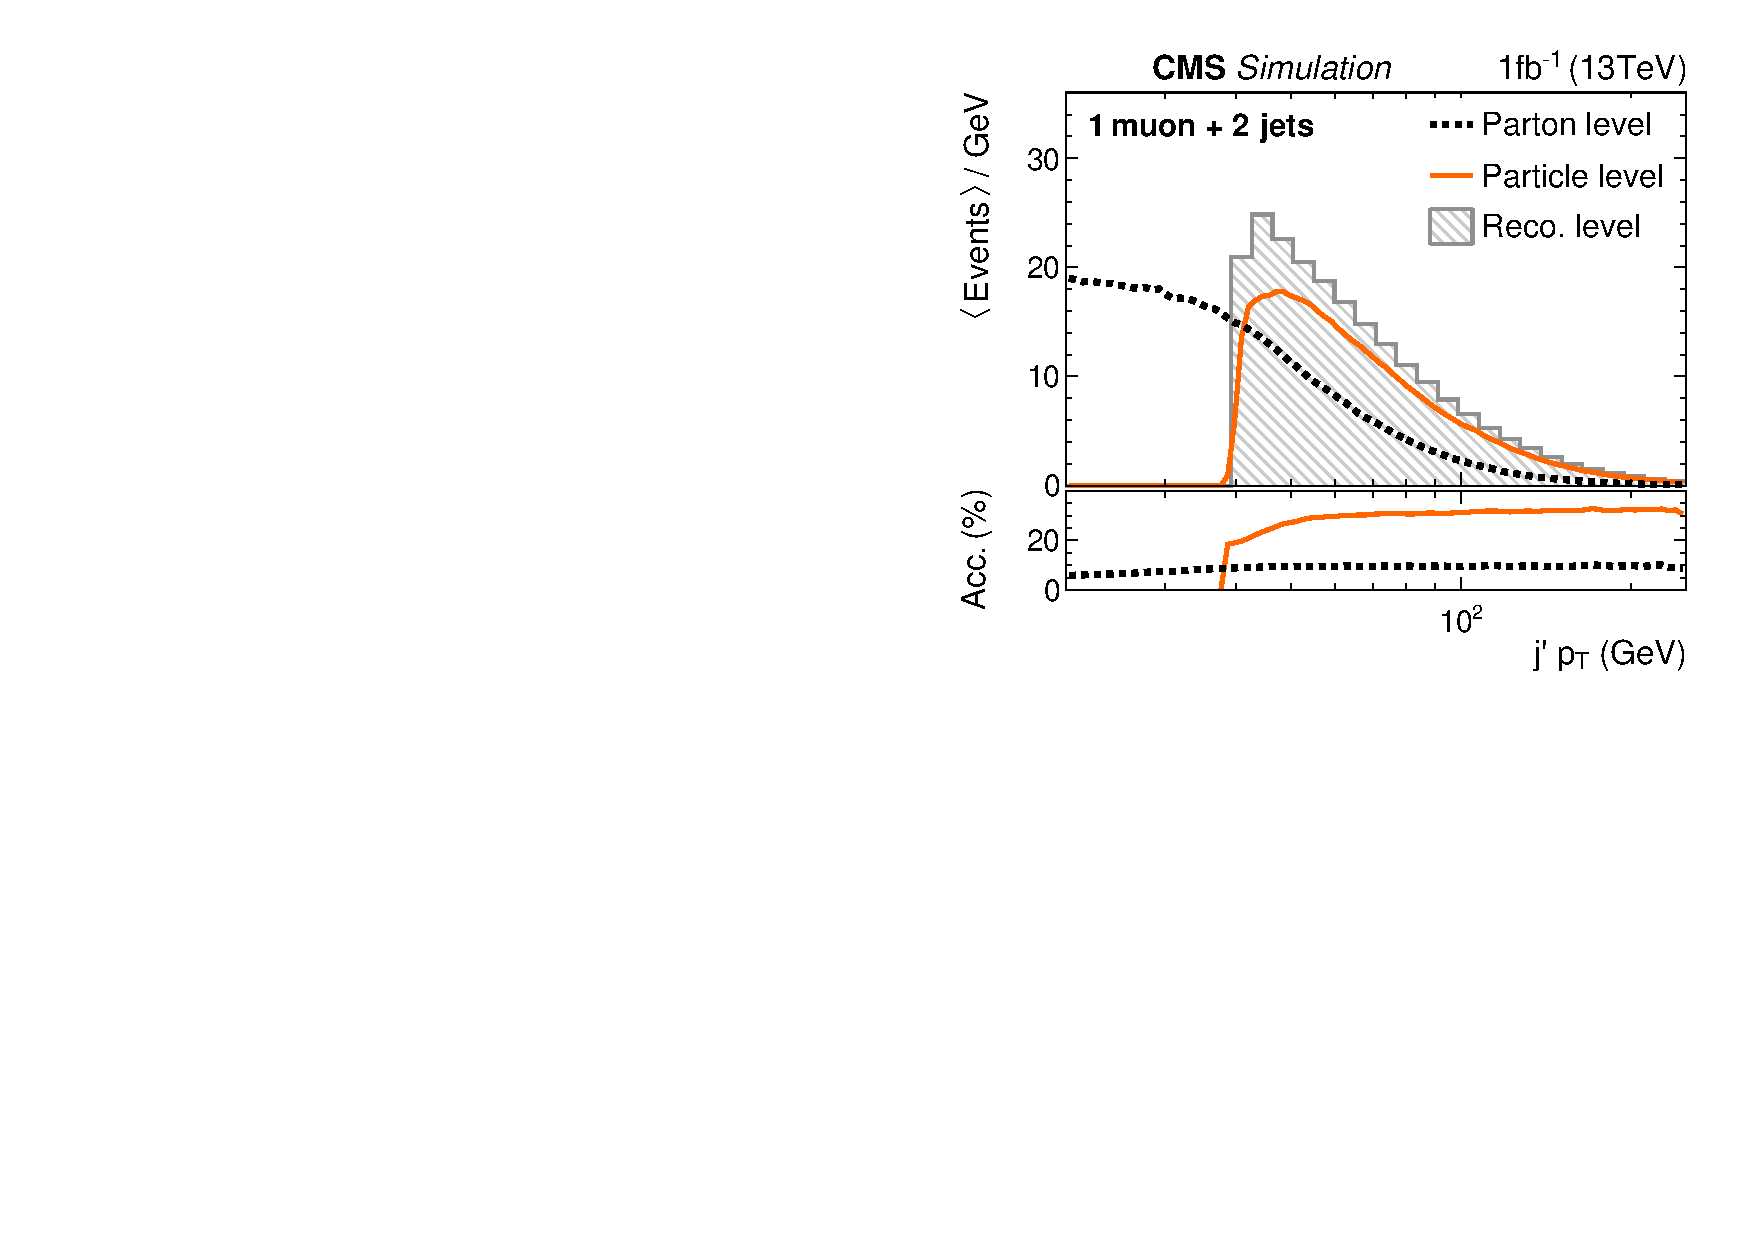
\includegraphics[width=0.48\textwidth]{figures/prospects/fiducial/ljet_particle_logpt.pdf}}\hspace{0.03\textwidth}
\subfloat[]{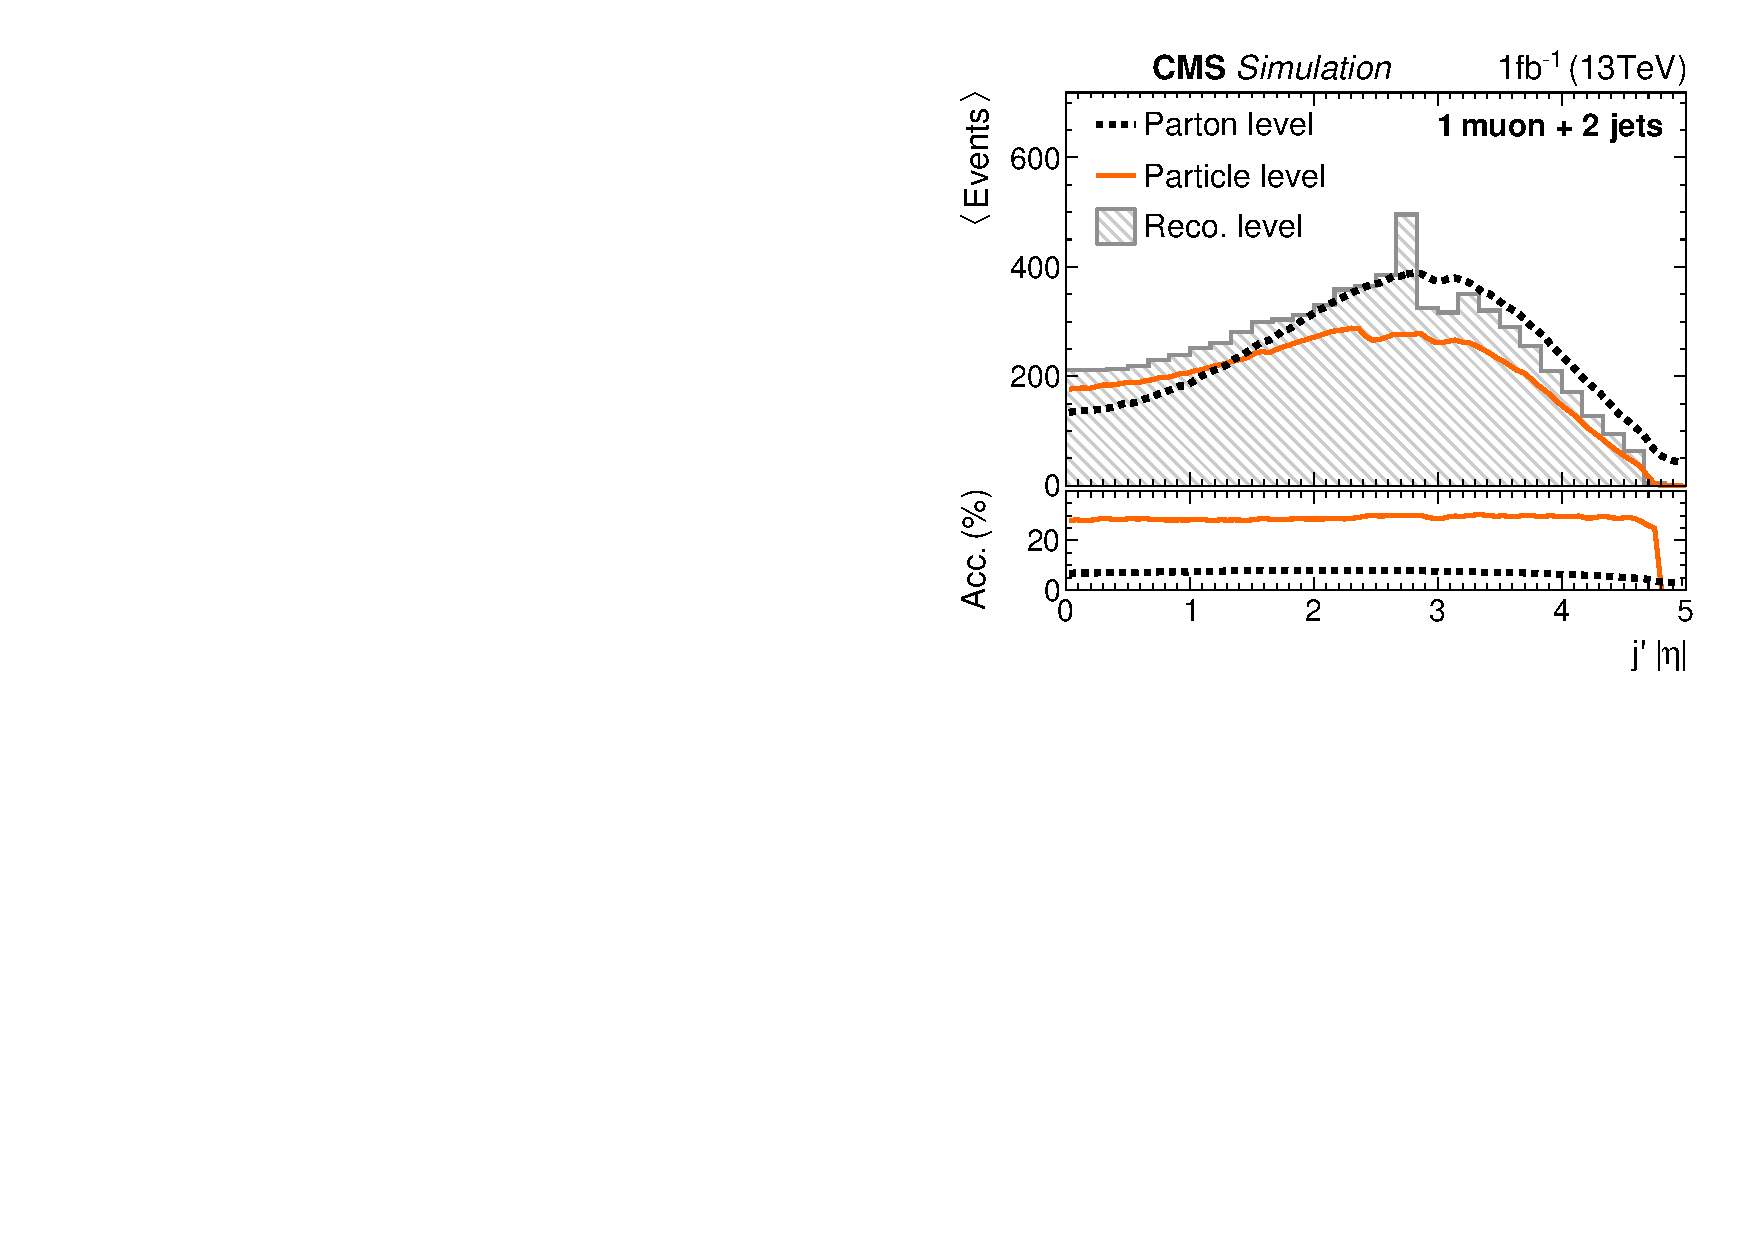
\includegraphics[width=0.48\textwidth]{figures/prospects/fiducial/ljet_particle_eta.pdf}}
}

Lastly, the distribution of the top quark polarization angle is shown in Fig.~\ref{fig:prospects-particle-cosTheta}. Its definition requires the full reconstruction and assignment of analysis objects to the $t$-channel single-top-quark signature. It is calculated as the angle between the muon and the spectator jet in the top quark rest-frame. 
The drop at $\cos\theta_\mu^\star\to1$ occurs mainly due to the applied \pt threshold on the selected muon as detailed in Sec.~\ref{sec:technique-levels}. The drop vanishes in the inclusive phase space at parton level. Hence, measuring the polarization angle angle at the particle level would particularly benefit from the reduced extrapolation into the fiducial phase space.

\myfigure{\label{fig:prospects-particle-cosTheta}Distribution of the top quark polarization angle. Top panel: common events selected at reconstruction level; bottom panel: acceptance of reconstruction level selection. The figure is taken from Ref.~\cite{particleStudies}.}{
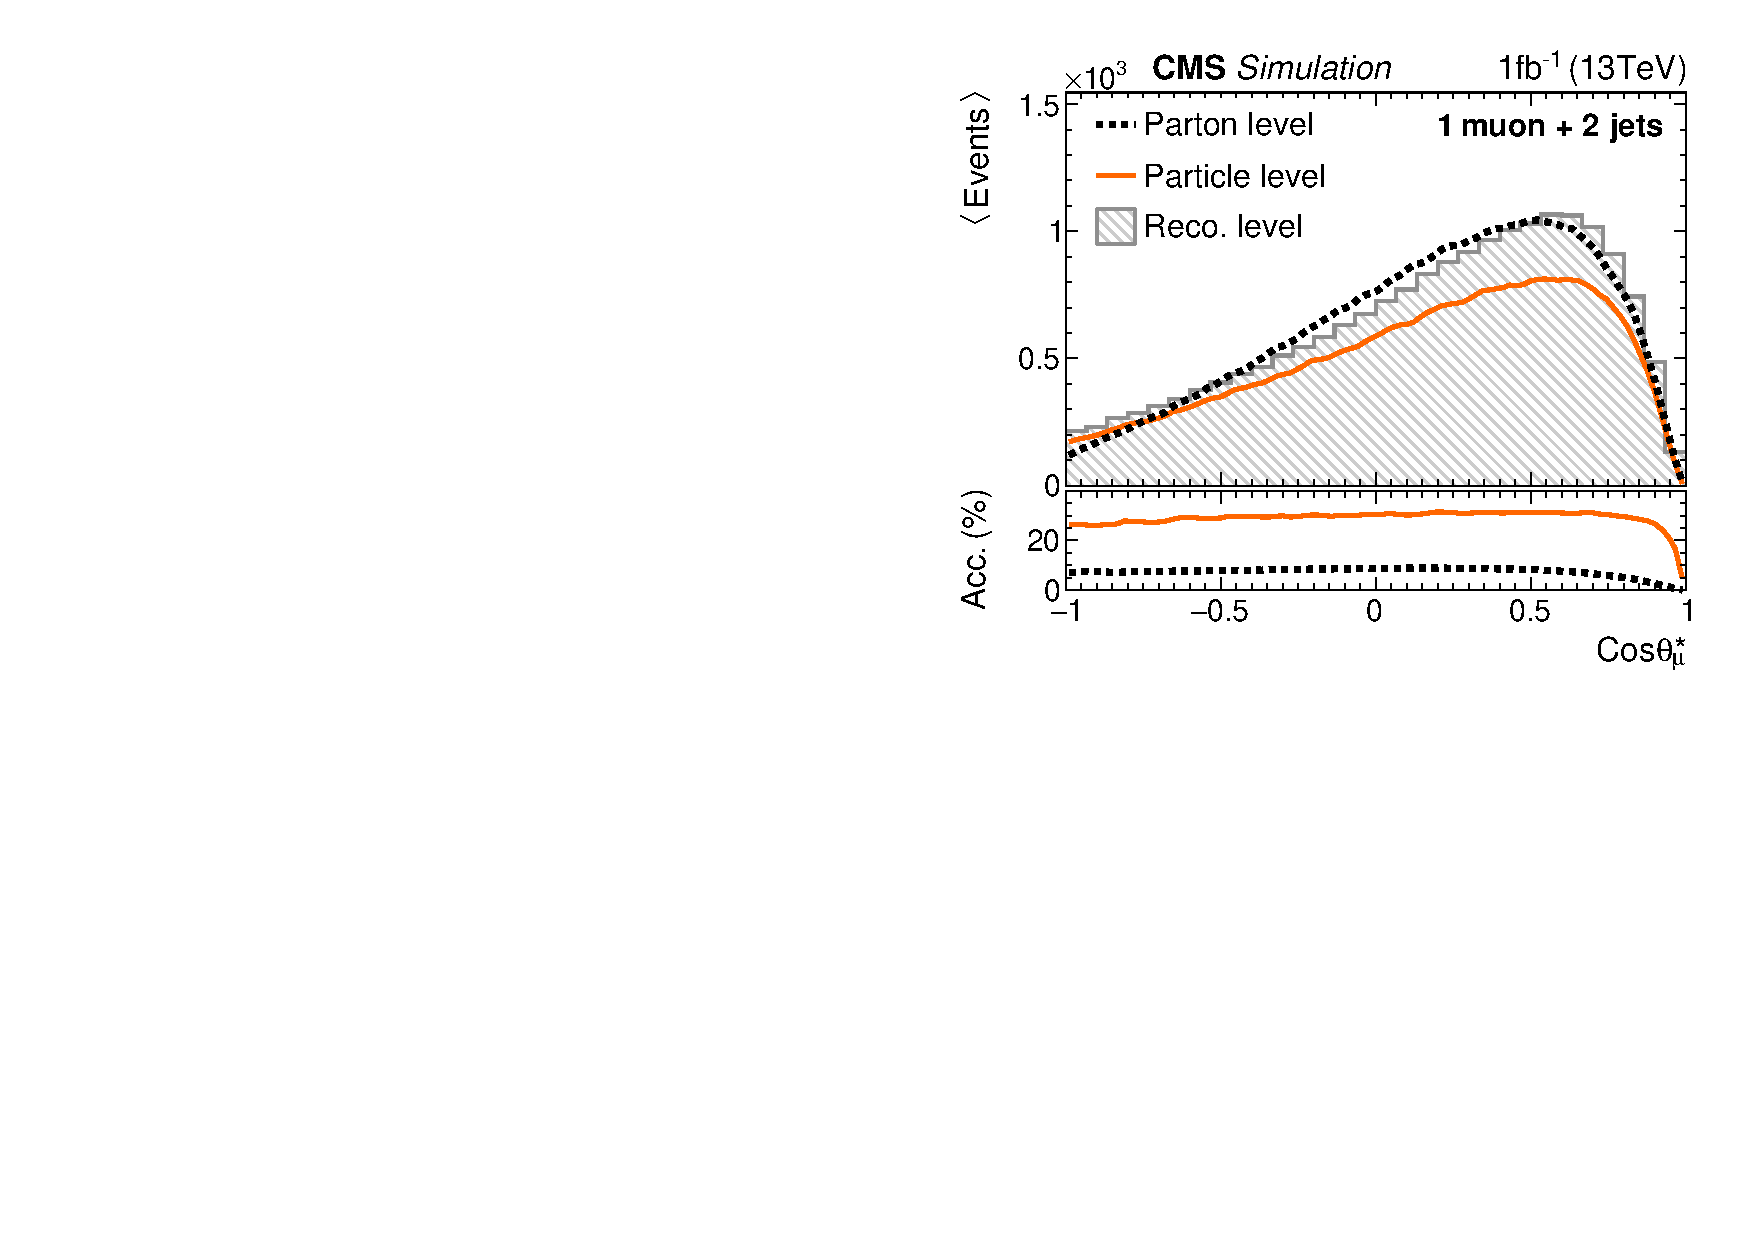
\includegraphics[width=0.48\textwidth]{figures/prospects/fiducial/cosTheta_particle.pdf}
}

%##############################################
\section{Unfolding and results}
%##############################################

The unfolding of pseudo-data to particle and parton level is demonstrated in the following. For this, distributions of pseudo-data of the \mtw, and the \bdttt and \bdttch discriminants are generated from the simulated samples and the multijet template. In addition a random Poisson fluctuation corresponding to the expected number of data events is applied per bin. The distributions are obtained in 12 independent intervals per top quark \pt, rapidity, or polarization angle for fitting. The estimated signal scale factors are passed to the unfolding. Only six bins are considered at particle or parton level to stabilize the minimization within the \TUNFOLD unfolding procedure. Response matrices for unfolding to parton or particle level are constructed from simulated $t$-channel single-top-quark events. The obtained matrices in the muon channel are presented in Fig.~\ref{fig:prospects-response}. The migrations between bins are significantly reduced when unfolding to particle level compared to parton level which is particularly visible for the polarization angle.

\myfigure[p]{\label{fig:prospects-response}Response matrices in muon channel for (left column)~particle level and (right column)~parton level: (top row)~top quark \pt; (middle row)~top quark rapidity; (bottom row)~polarization angle.}{
\subfloat[]{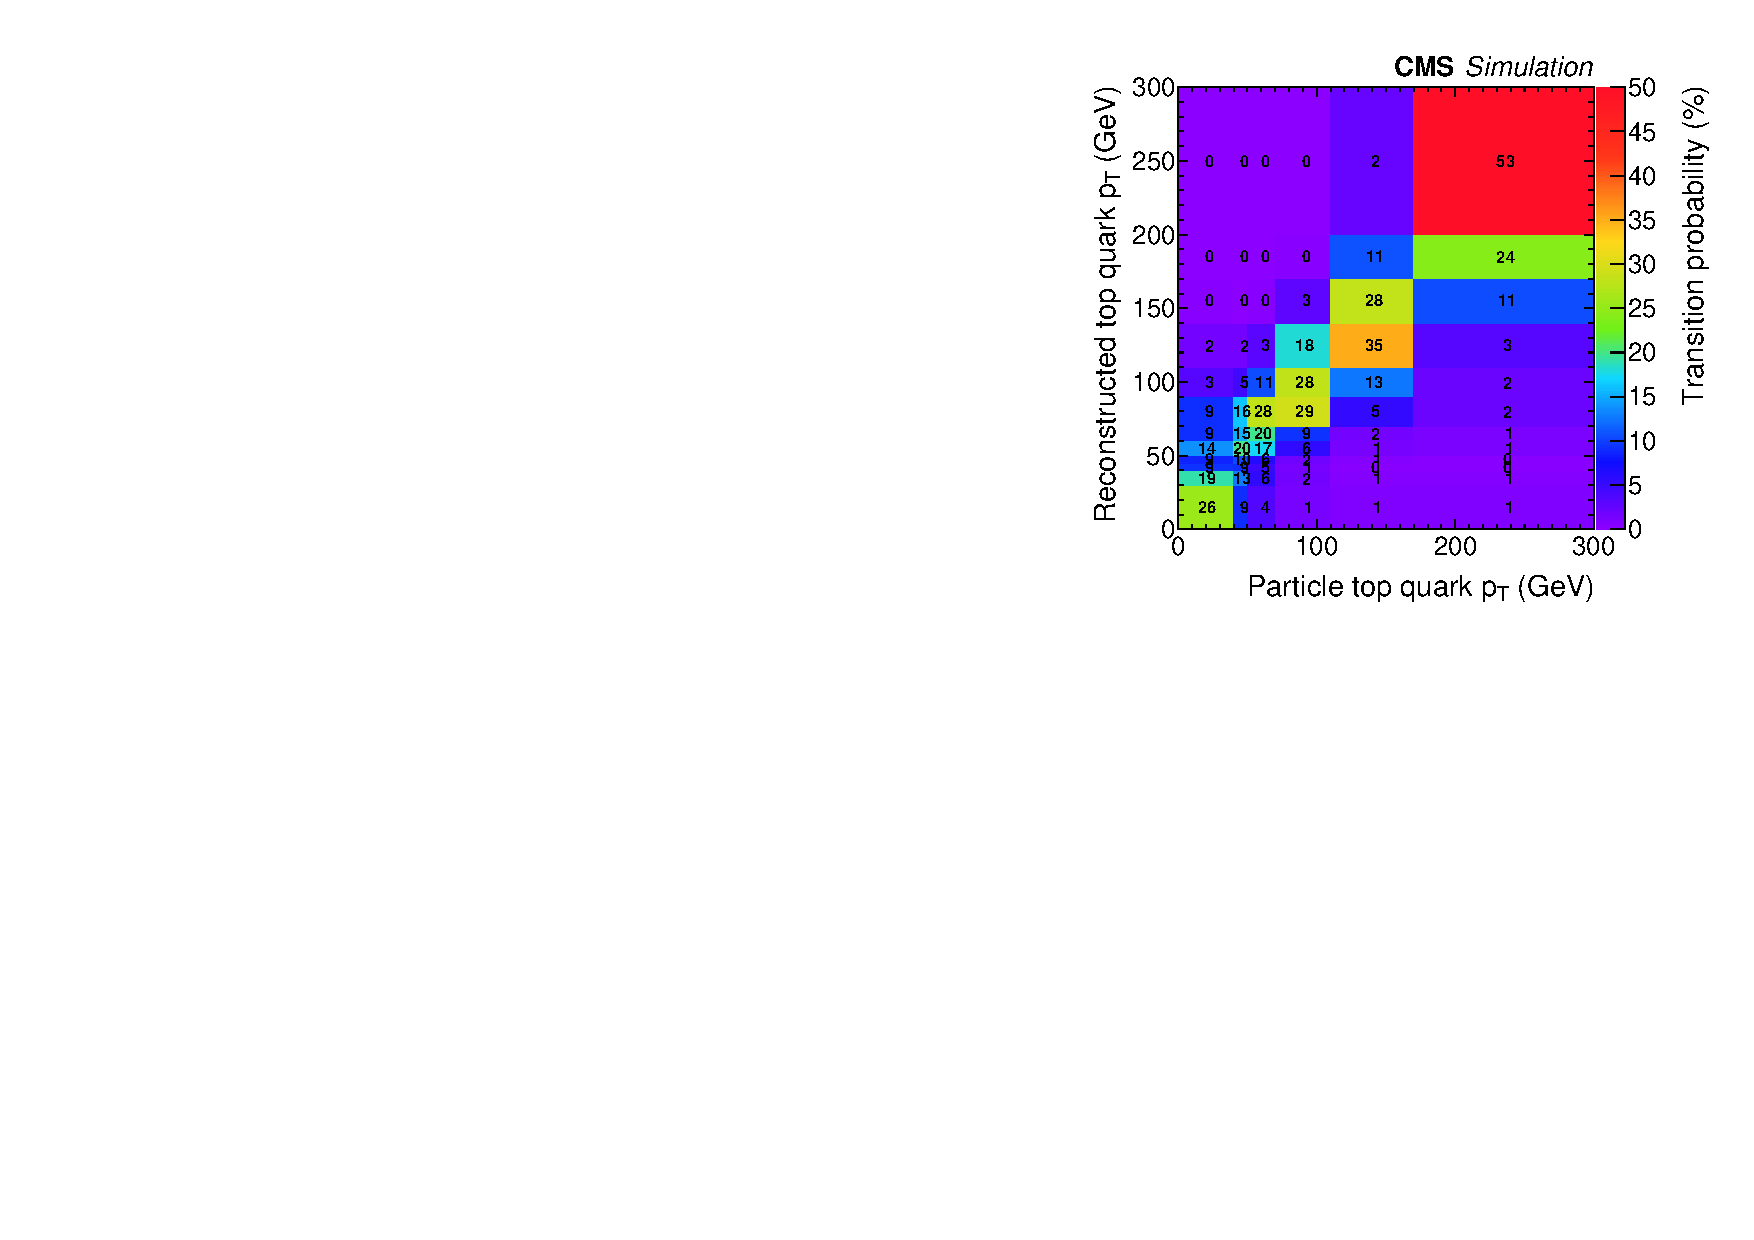
\includegraphics[width=0.48\textwidth]{figures/prospects/unfolding/responsePartilce_mu_pt.pdf}}\hspace{0.02\textwidth}
\subfloat[]{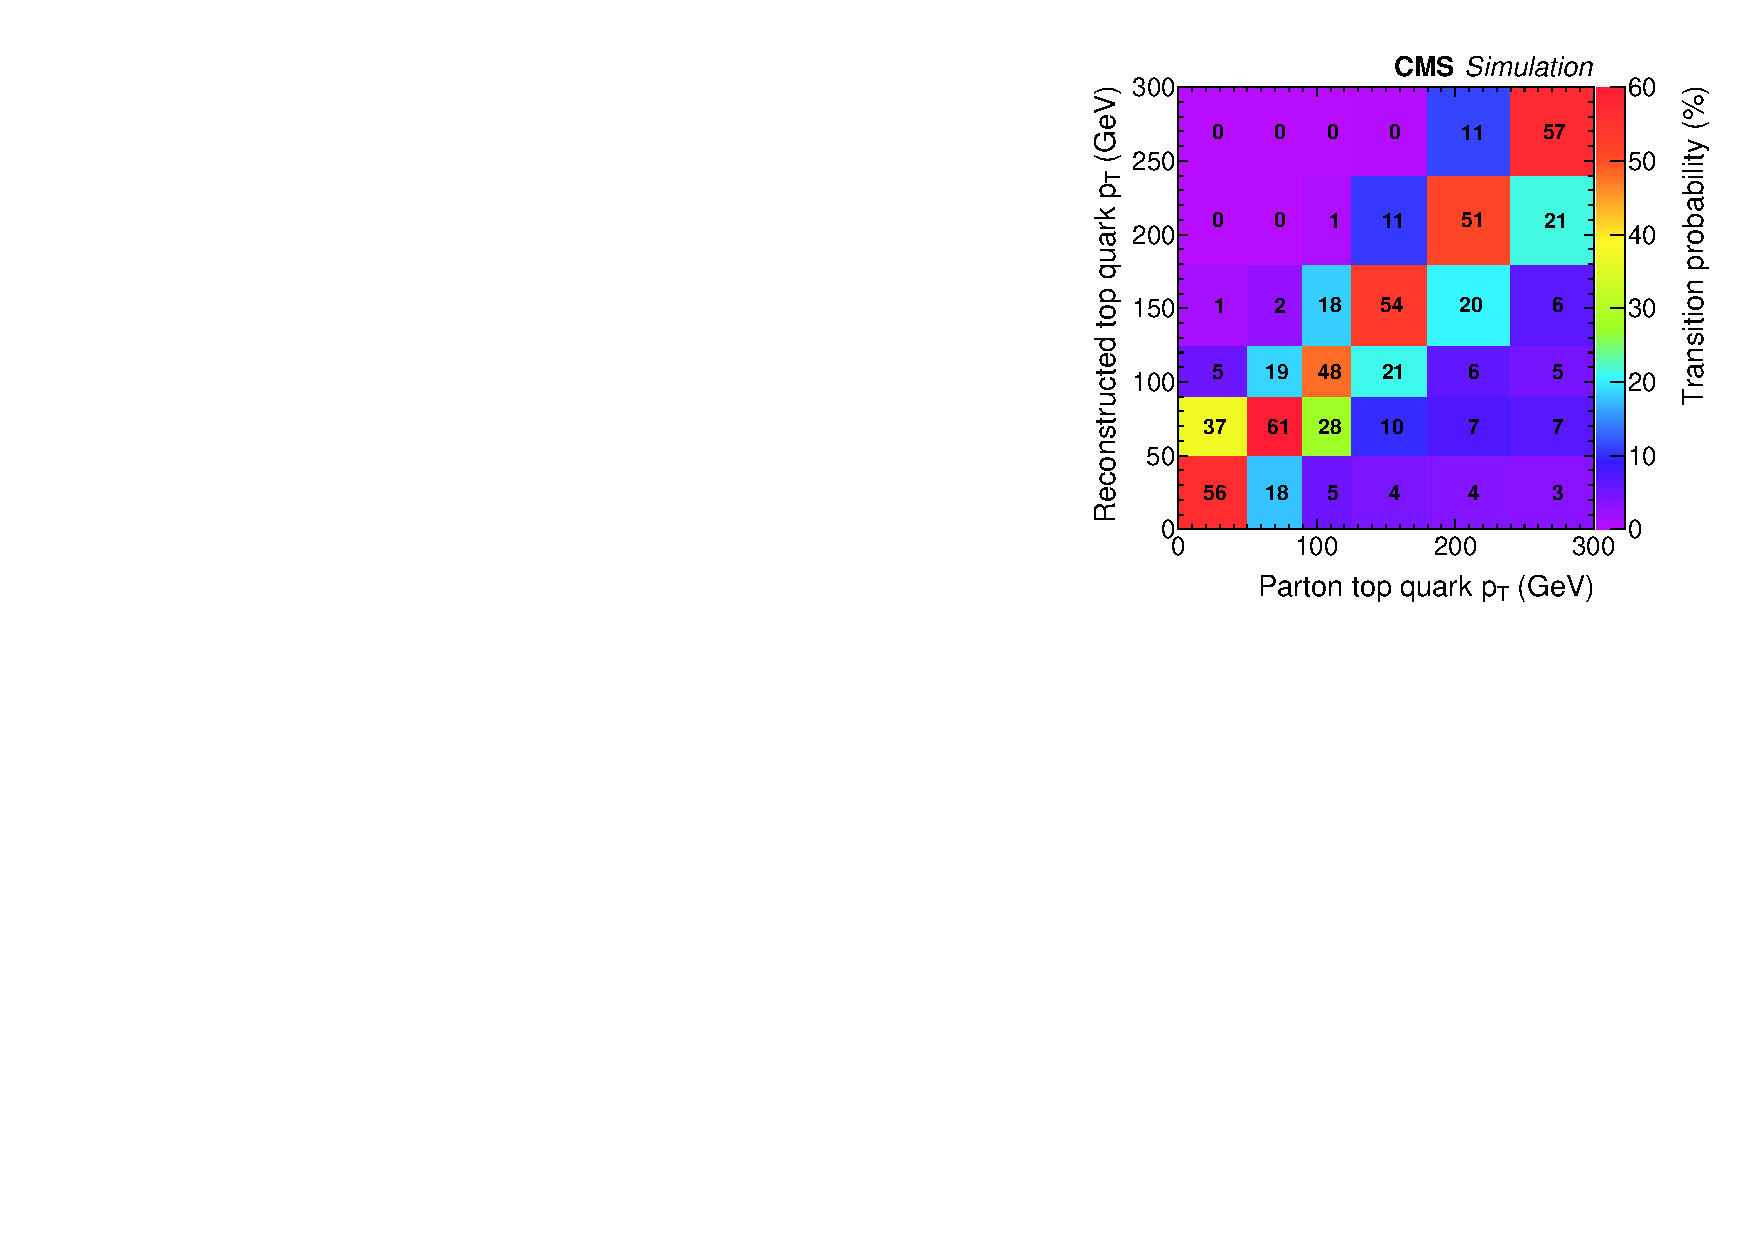
\includegraphics[width=0.48\textwidth]{figures/prospects/unfolding/responseParton_mu_pt.pdf}}\\
\subfloat[]{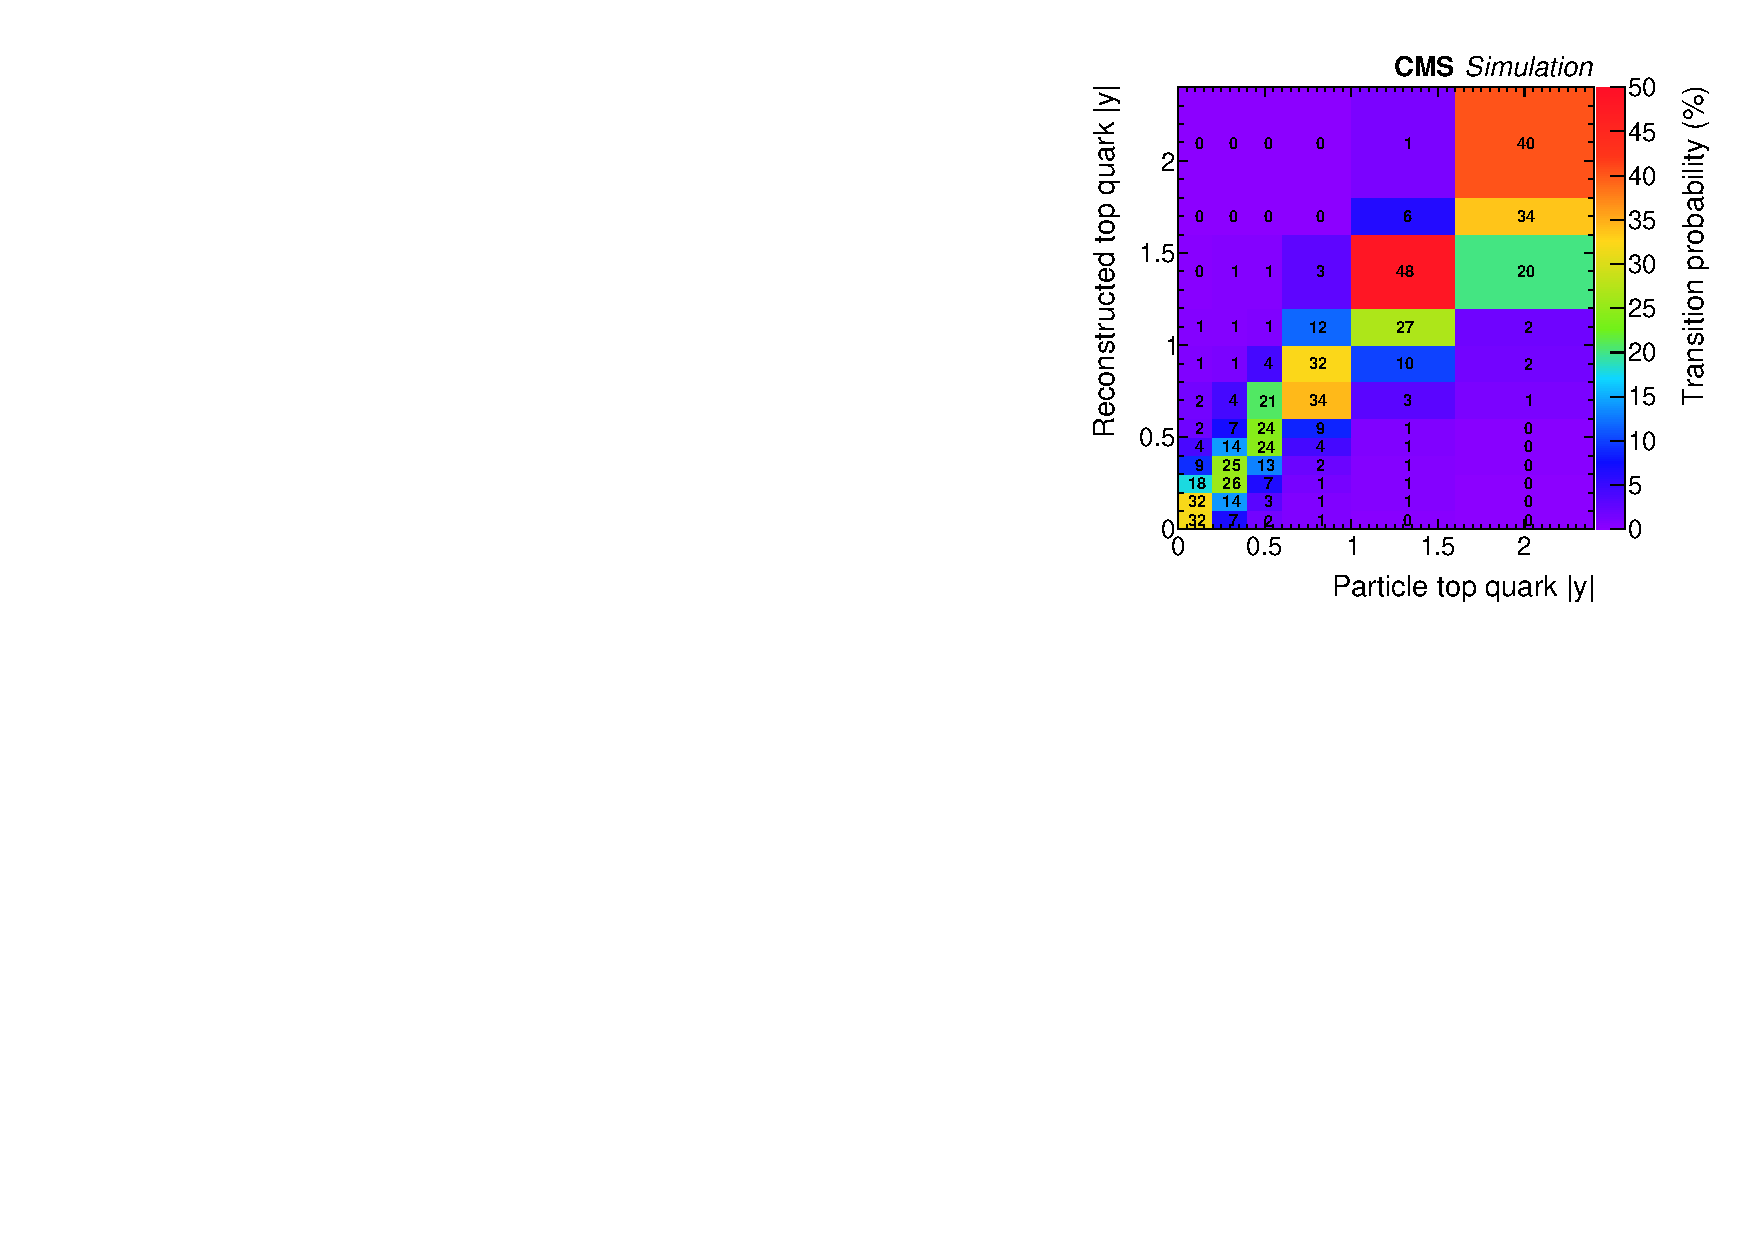
\includegraphics[width=0.48\textwidth]{figures/prospects/unfolding/responsePartilce_mu_y.pdf}}\hspace{0.02\textwidth}
\subfloat[]{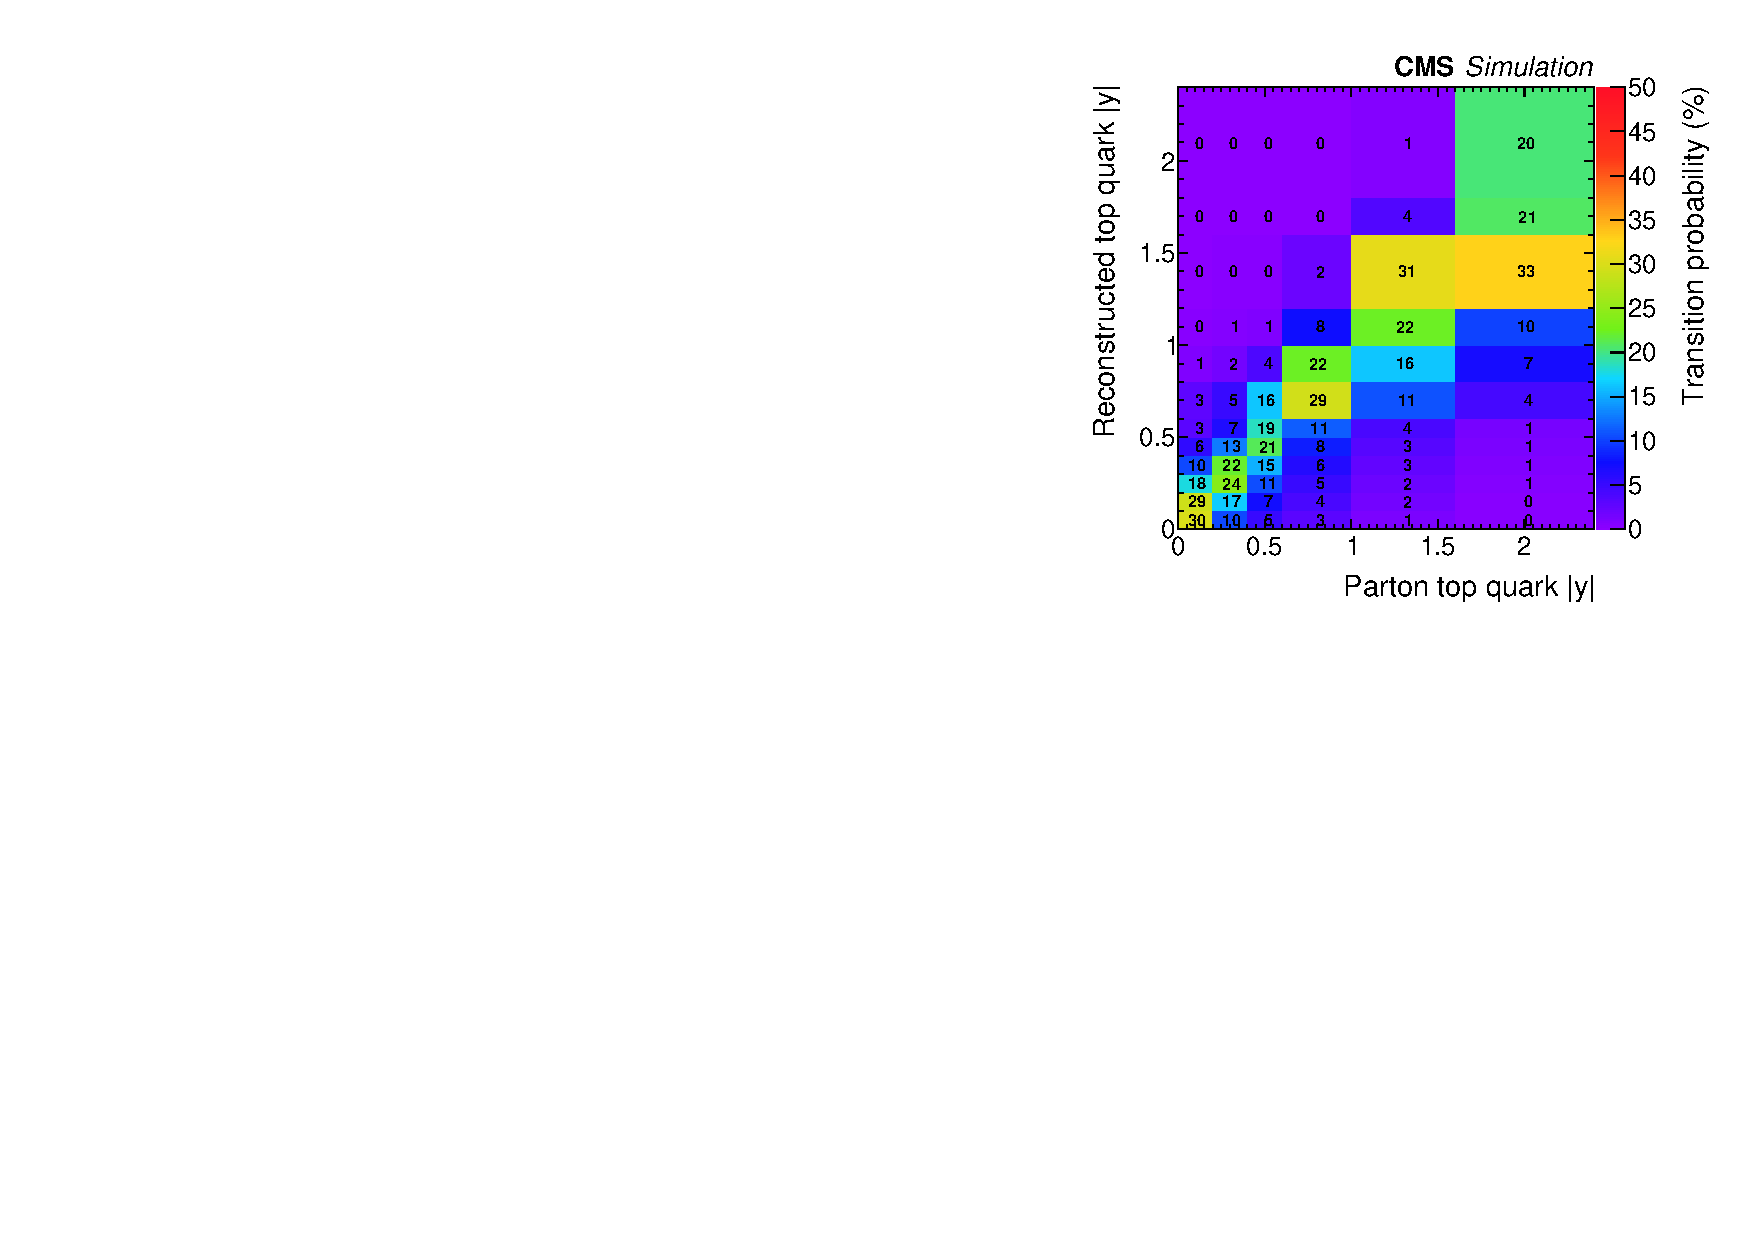
\includegraphics[width=0.48\textwidth]{figures/prospects/unfolding/responseParton_mu_y.pdf}}\\
\subfloat[]{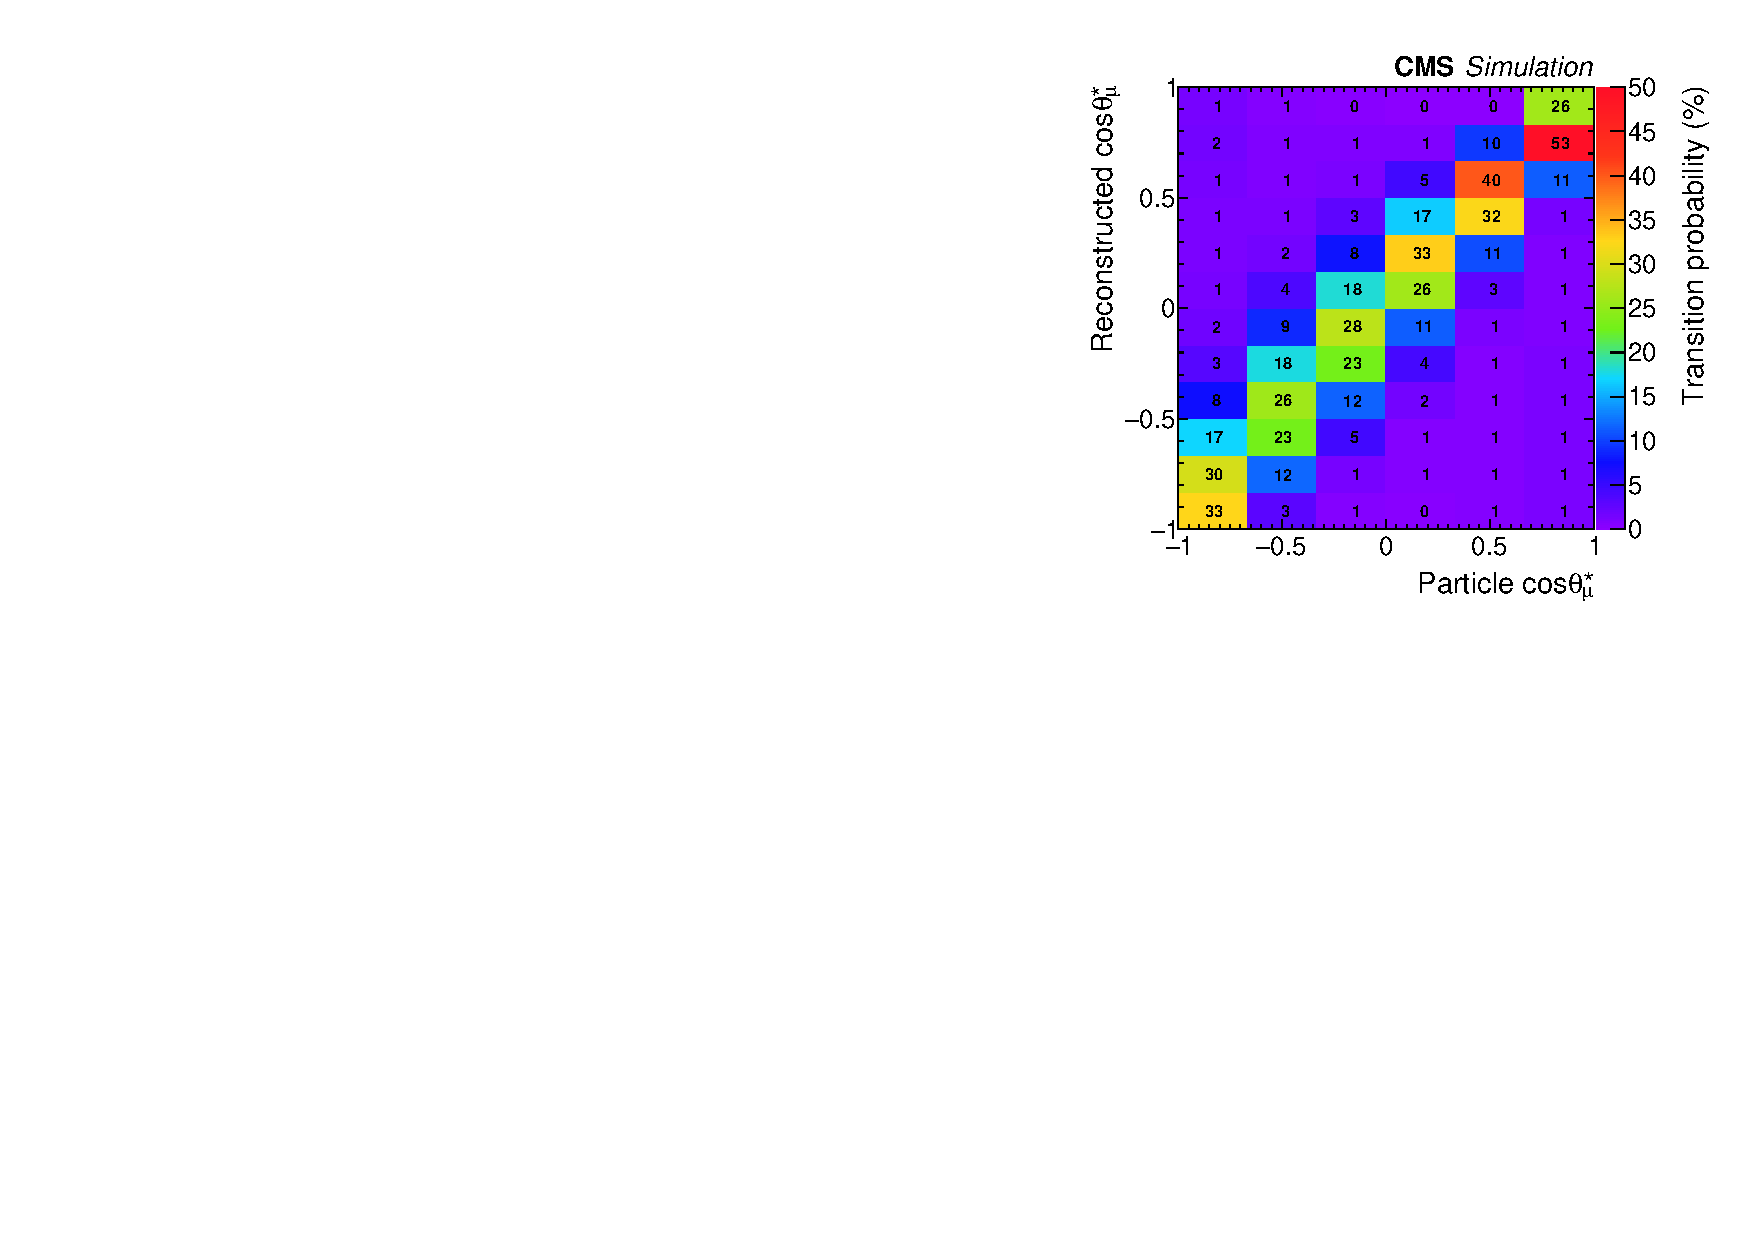
\includegraphics[width=0.48\textwidth]{figures/prospects/unfolding/responsePartilce_mu_cos.pdf}}\hspace{0.02\textwidth}
\subfloat[]{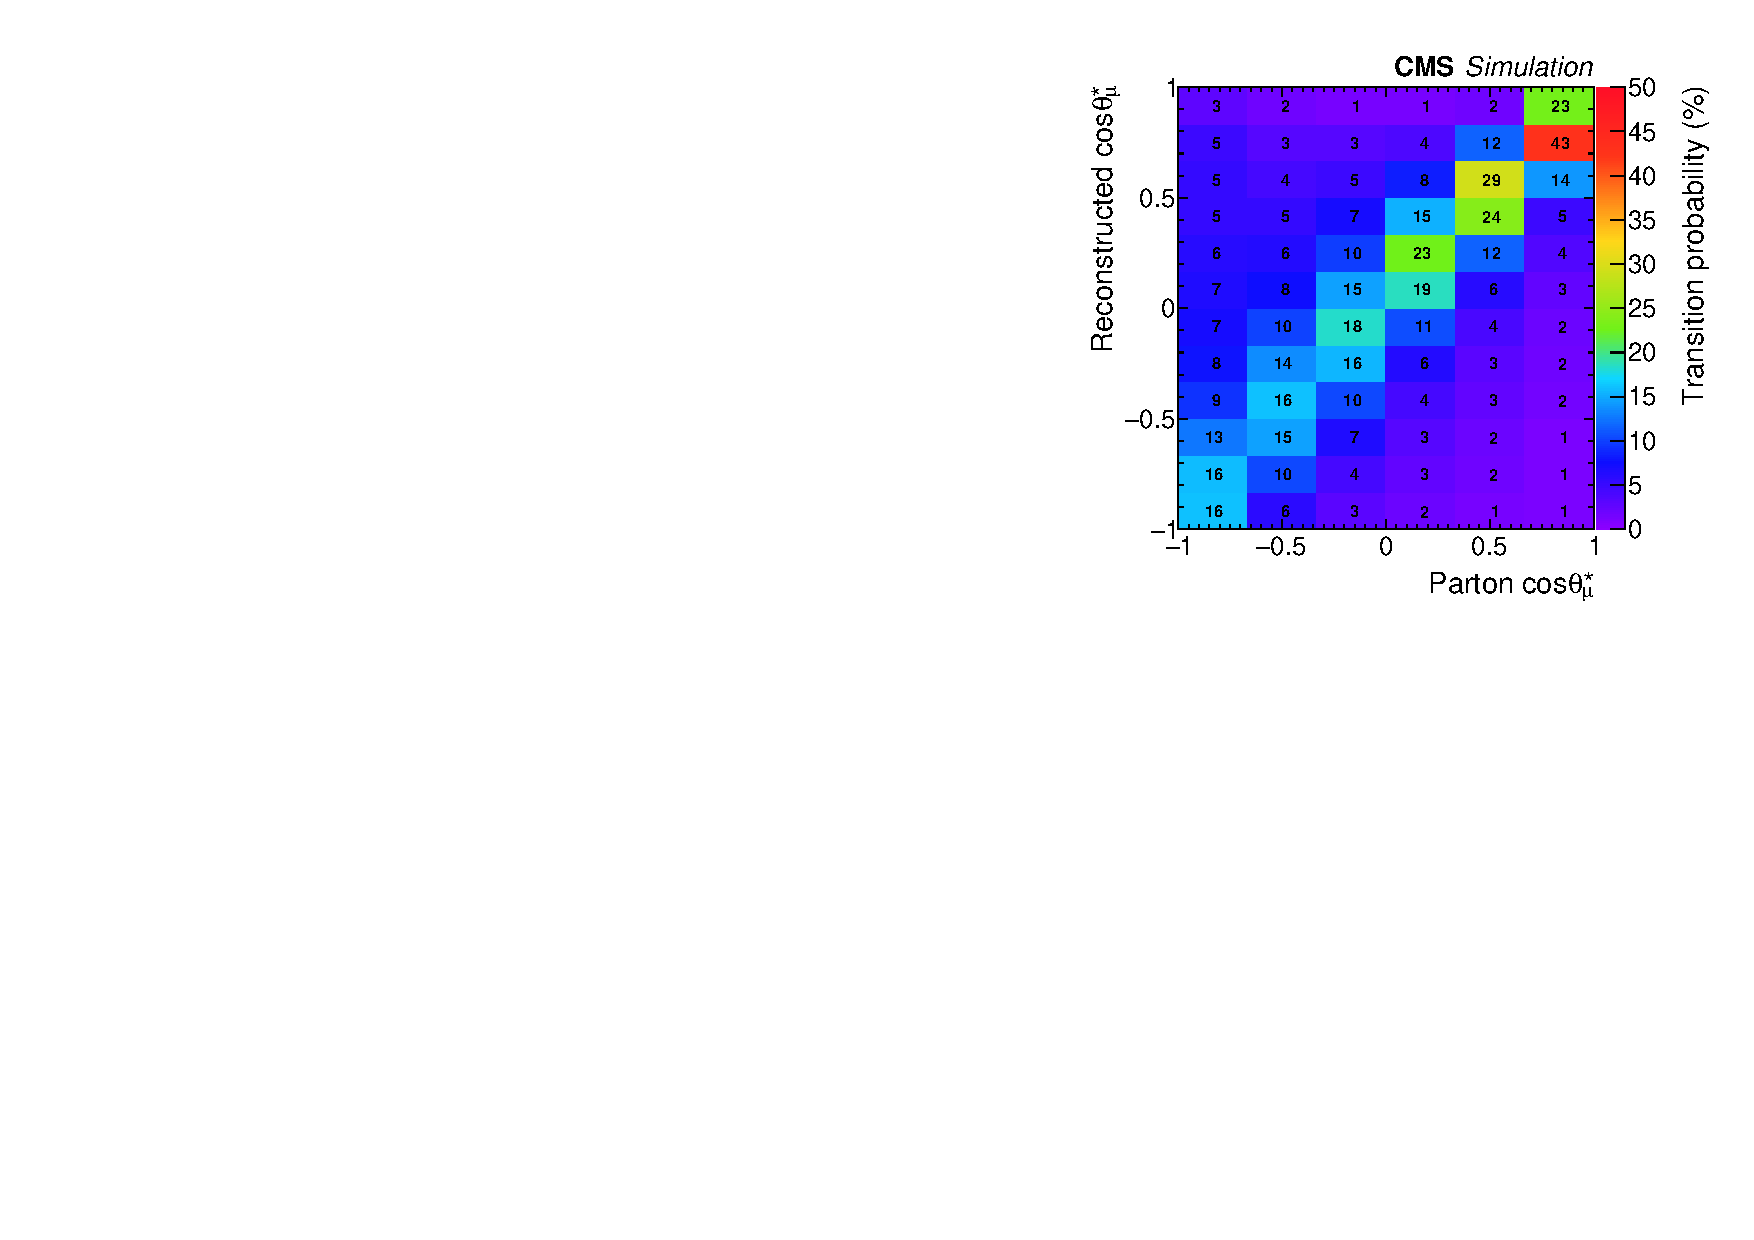
\includegraphics[width=0.48\textwidth]{figures/prospects/unfolding/responseParton_mu_cos.pdf}}
}

The resulting unfolded spectra in muon channel for the generated and fitted pseudo-data are presented in Fig.~\ref{fig:pospects-unfolded}. The indicated vertical bars reflect the expected statistical uncertainty on the estimated signal scale factor which has been propagated through the unfolding. Comparing the obtained spectra at particle and parton level side-by-side one can observe that the uncertainties in certain bins are largely increased at parton level compared to particle level which is a result of a low selection efficiency in those bins. This is in particular very significant for the first bin in the top quark \pt distribution and for the last bin in the distribution of the polarization angle. Thus, measuring differential cross sections at particle level as a function of these observables is clearly beneficial compared to parton level in terms of precision.

\myfigure[p]{\label{fig:pospects-unfolded}Unfolded distributions using pseudo-data in muon channel for (left column)~particle level and (right column)~parton level: (top row)~top quark \pt; (middle row)~top quark rapidity; (bottom row)~polarization angle. The vertical bar indicates the expected statistical uncertainty as propagated from the \gls{ml} fits.}{
\subfloat[]{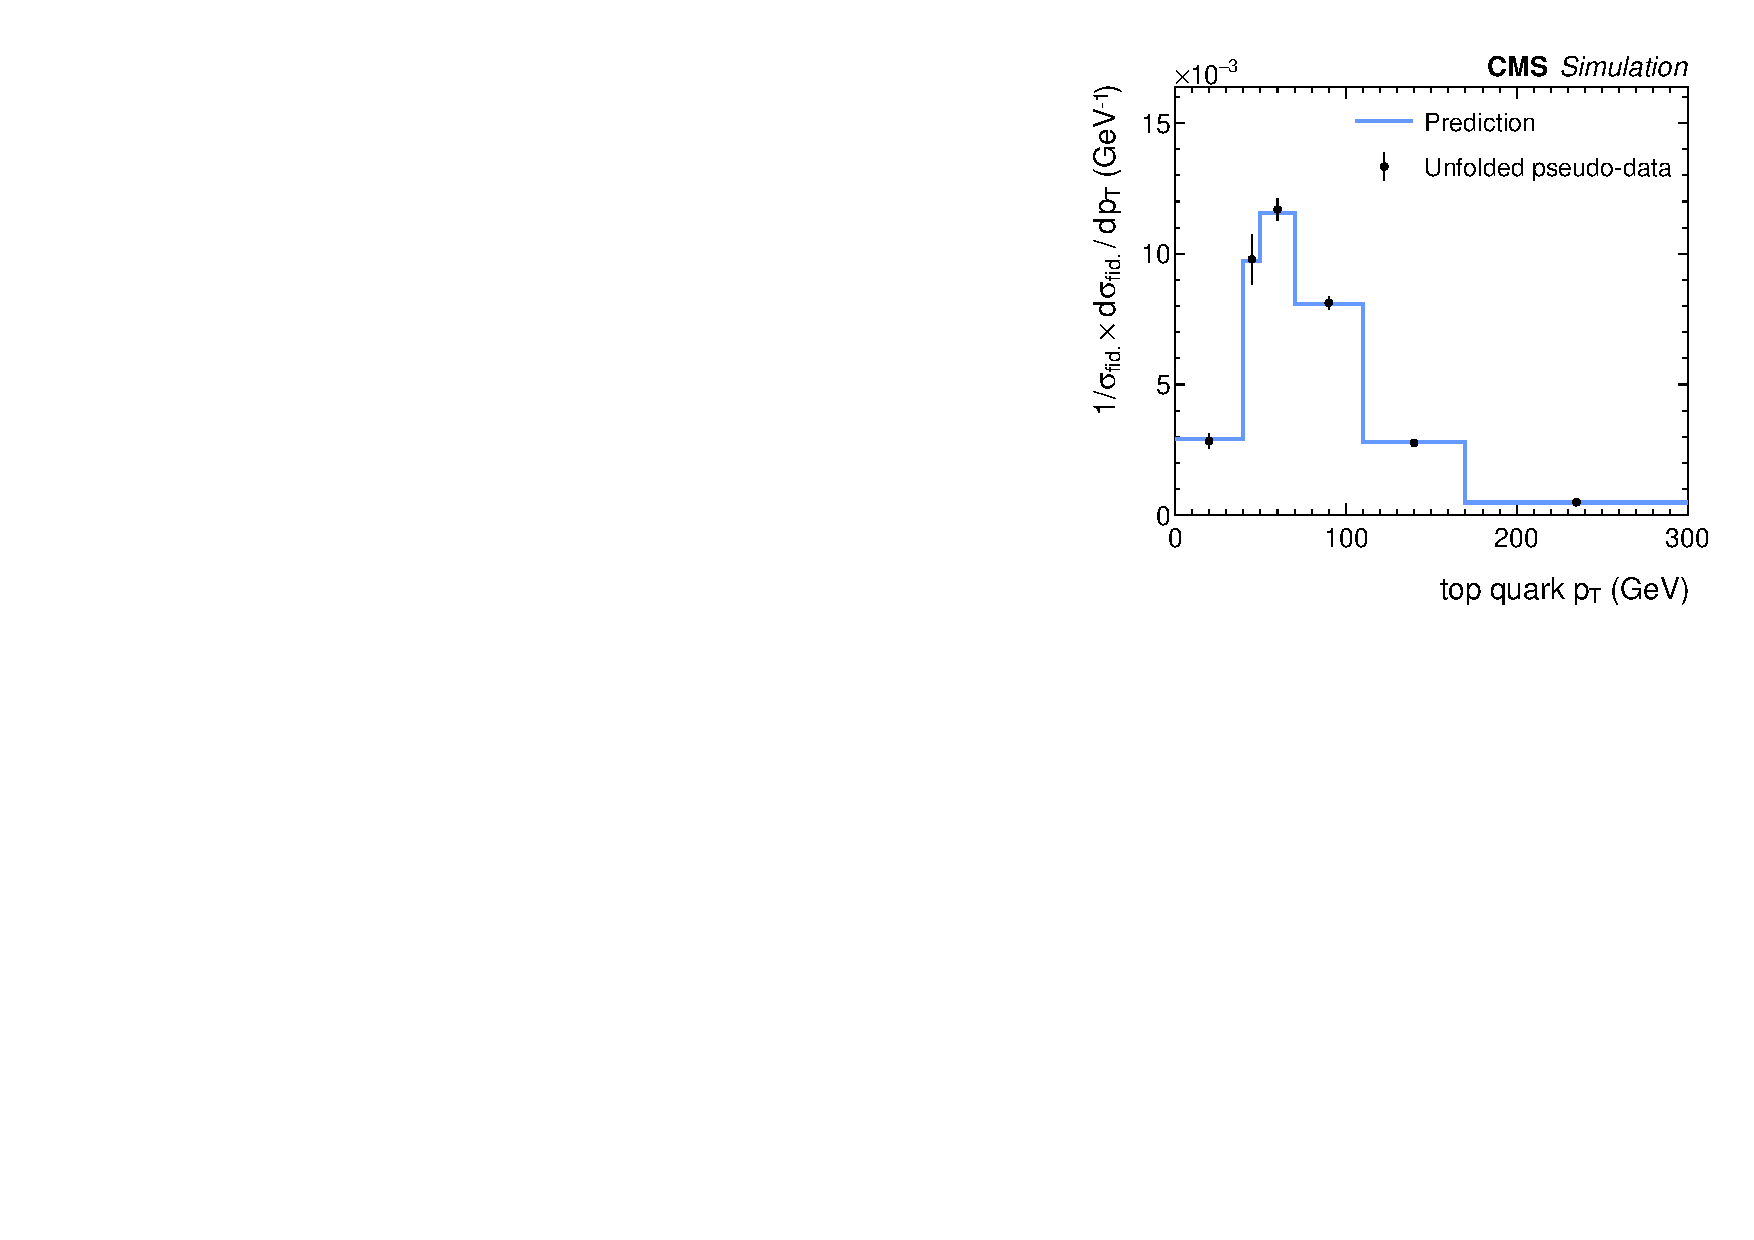
\includegraphics[width=0.48\textwidth]{figures/prospects/unfolding/unfoldedParticle_mu_pt.pdf}}\hspace{0.02\textwidth}
\subfloat[]{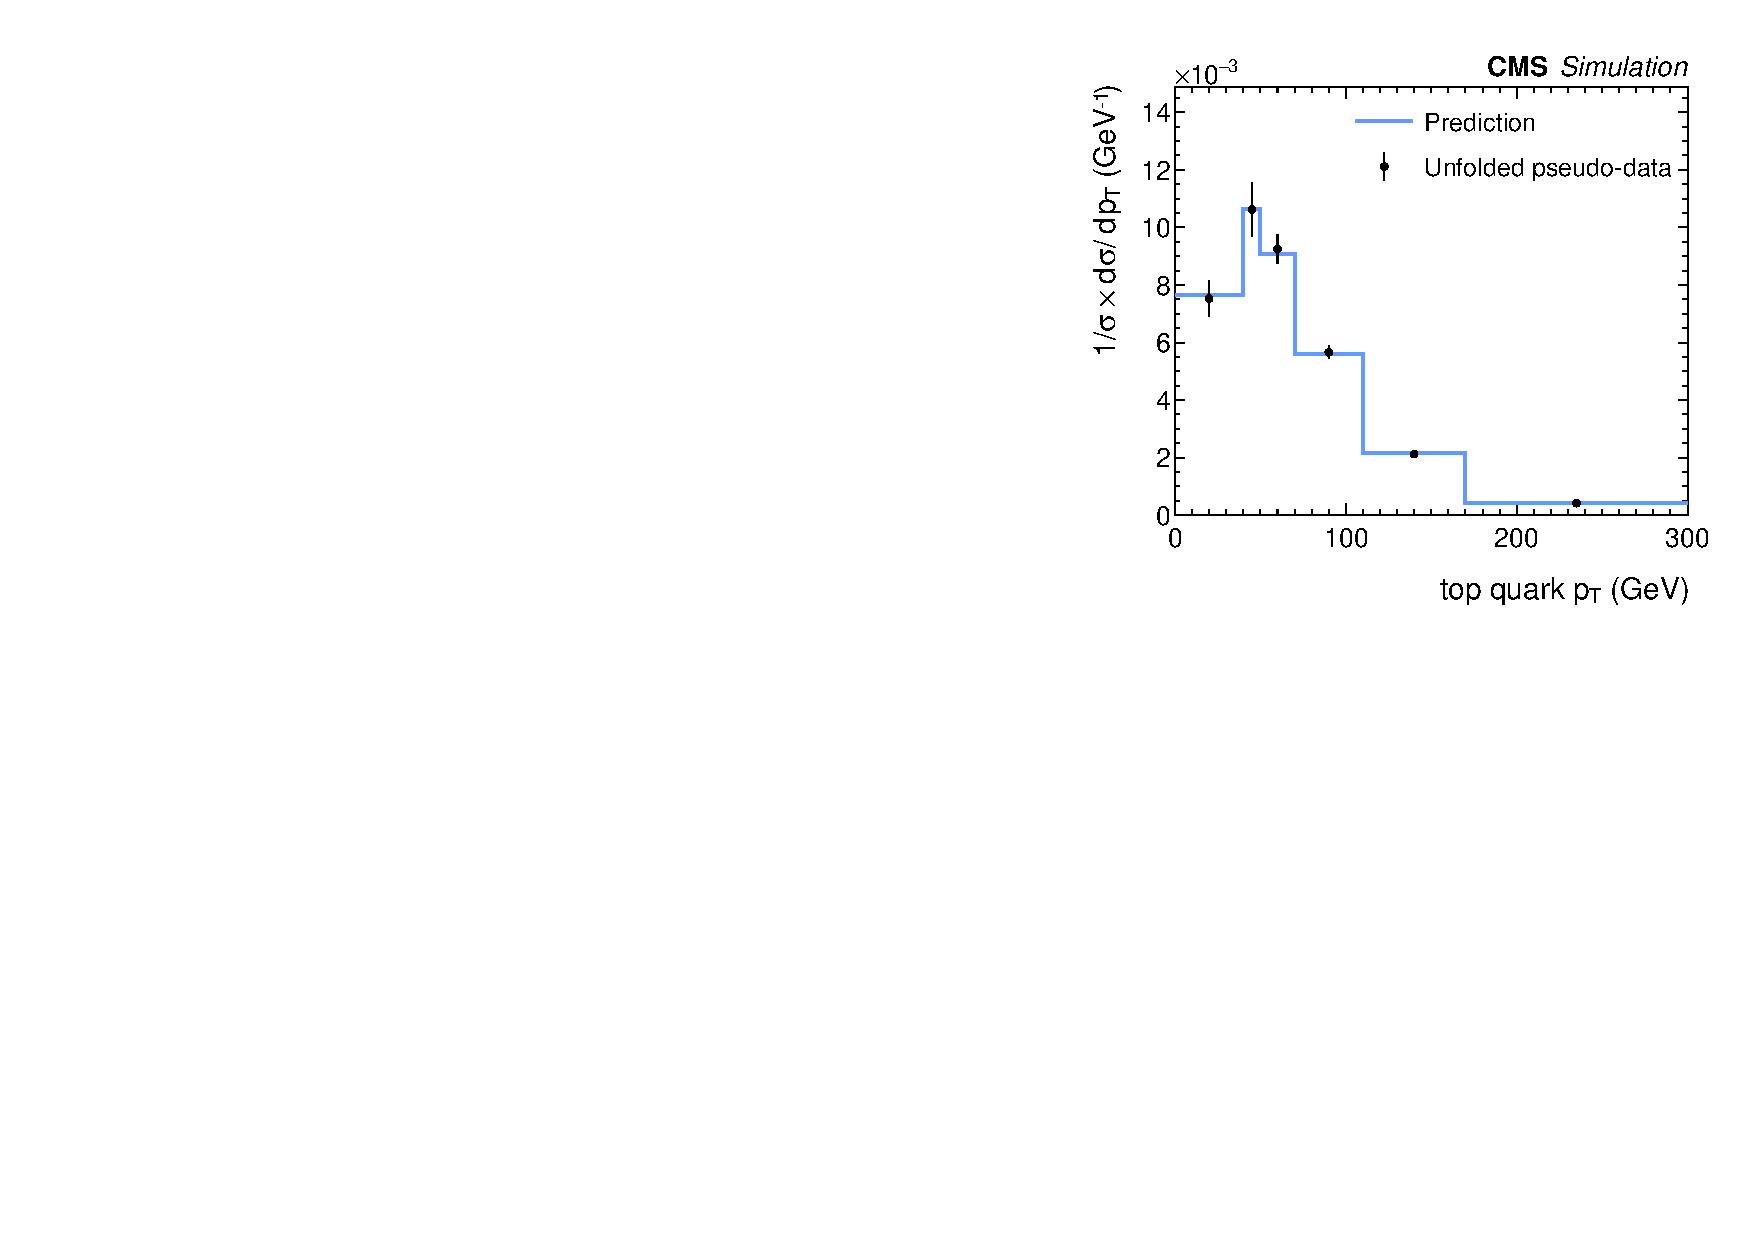
\includegraphics[width=0.48\textwidth]{figures/prospects/unfolding/unfoldedParton_mu_pt.pdf}}\\
\subfloat[]{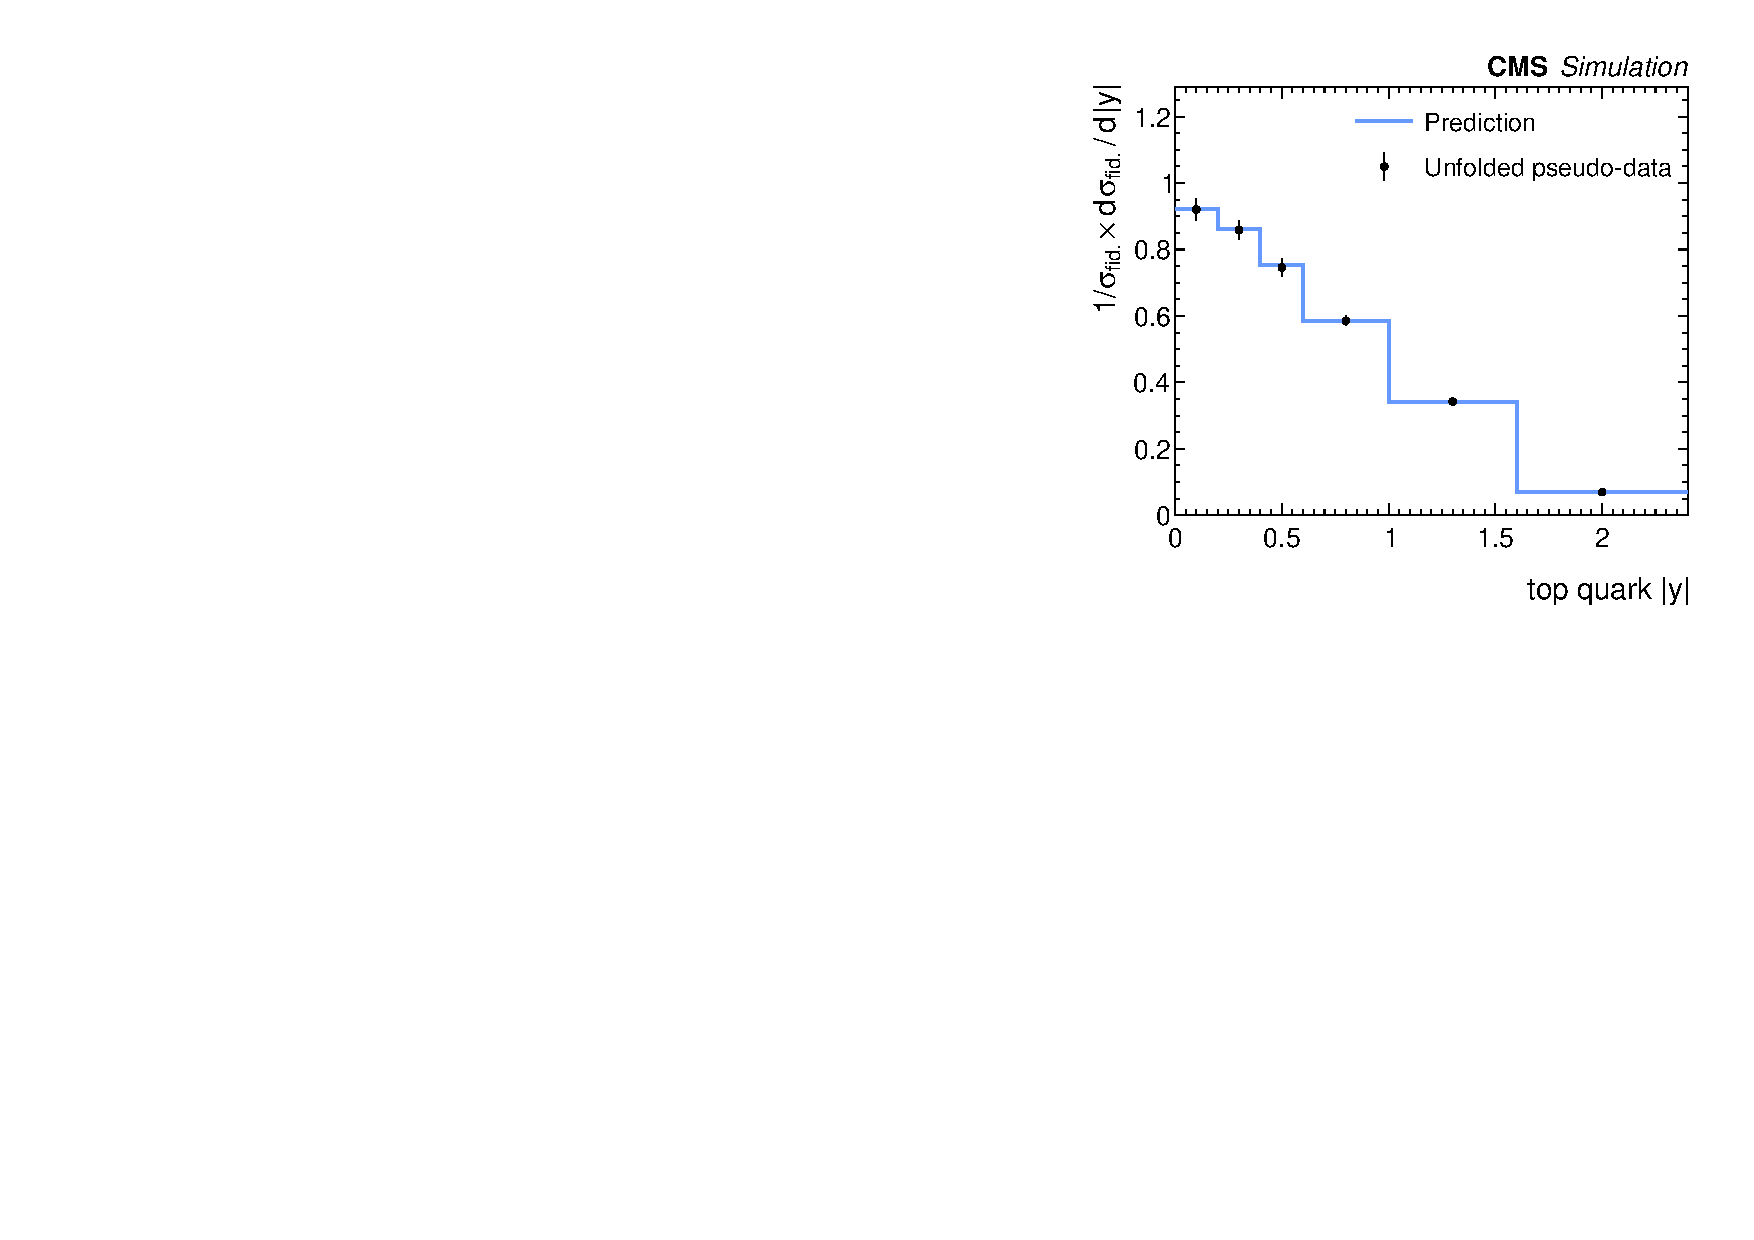
\includegraphics[width=0.48\textwidth]{figures/prospects/unfolding/unfoldedParticle_mu_y.pdf}}\hspace{0.02\textwidth}
\subfloat[]{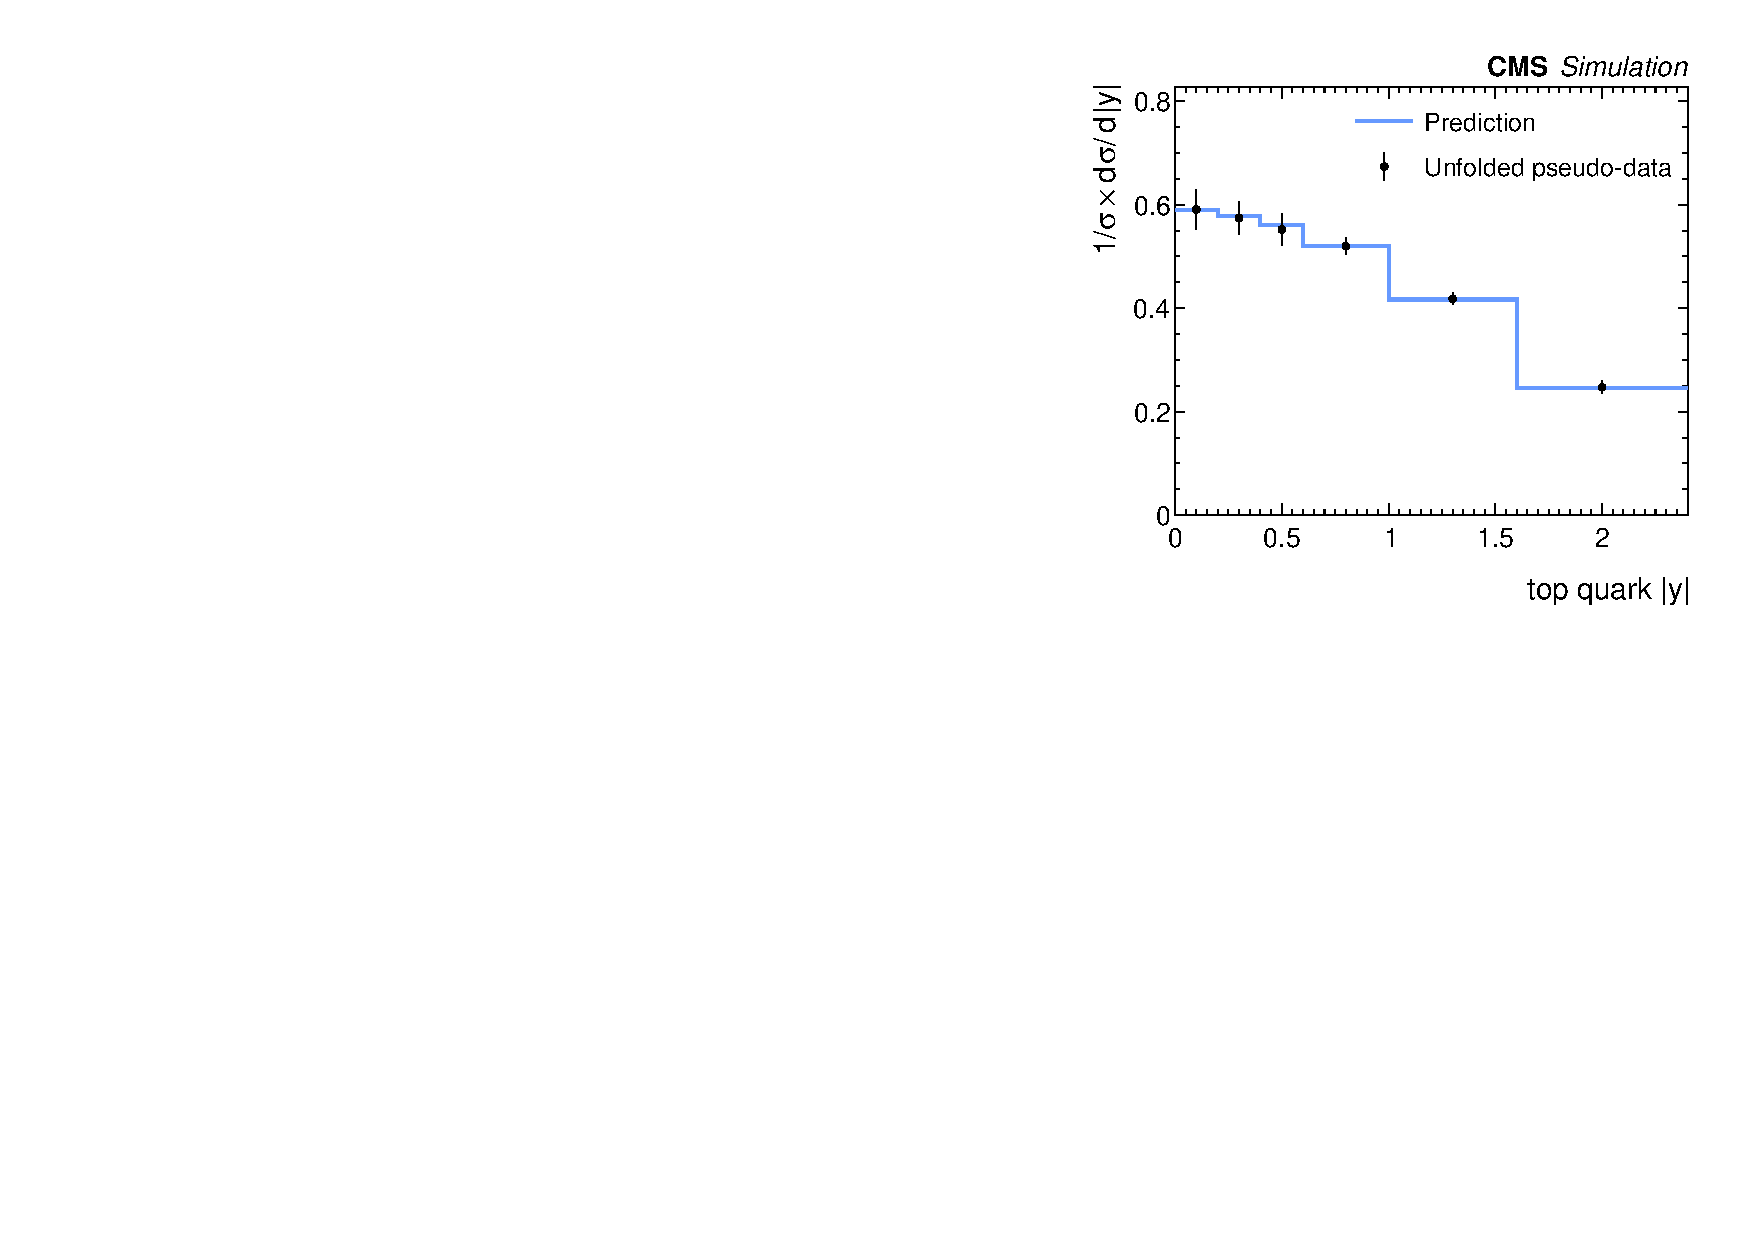
\includegraphics[width=0.48\textwidth]{figures/prospects/unfolding/unfoldedParton_mu_y.pdf}}\\
\subfloat[]{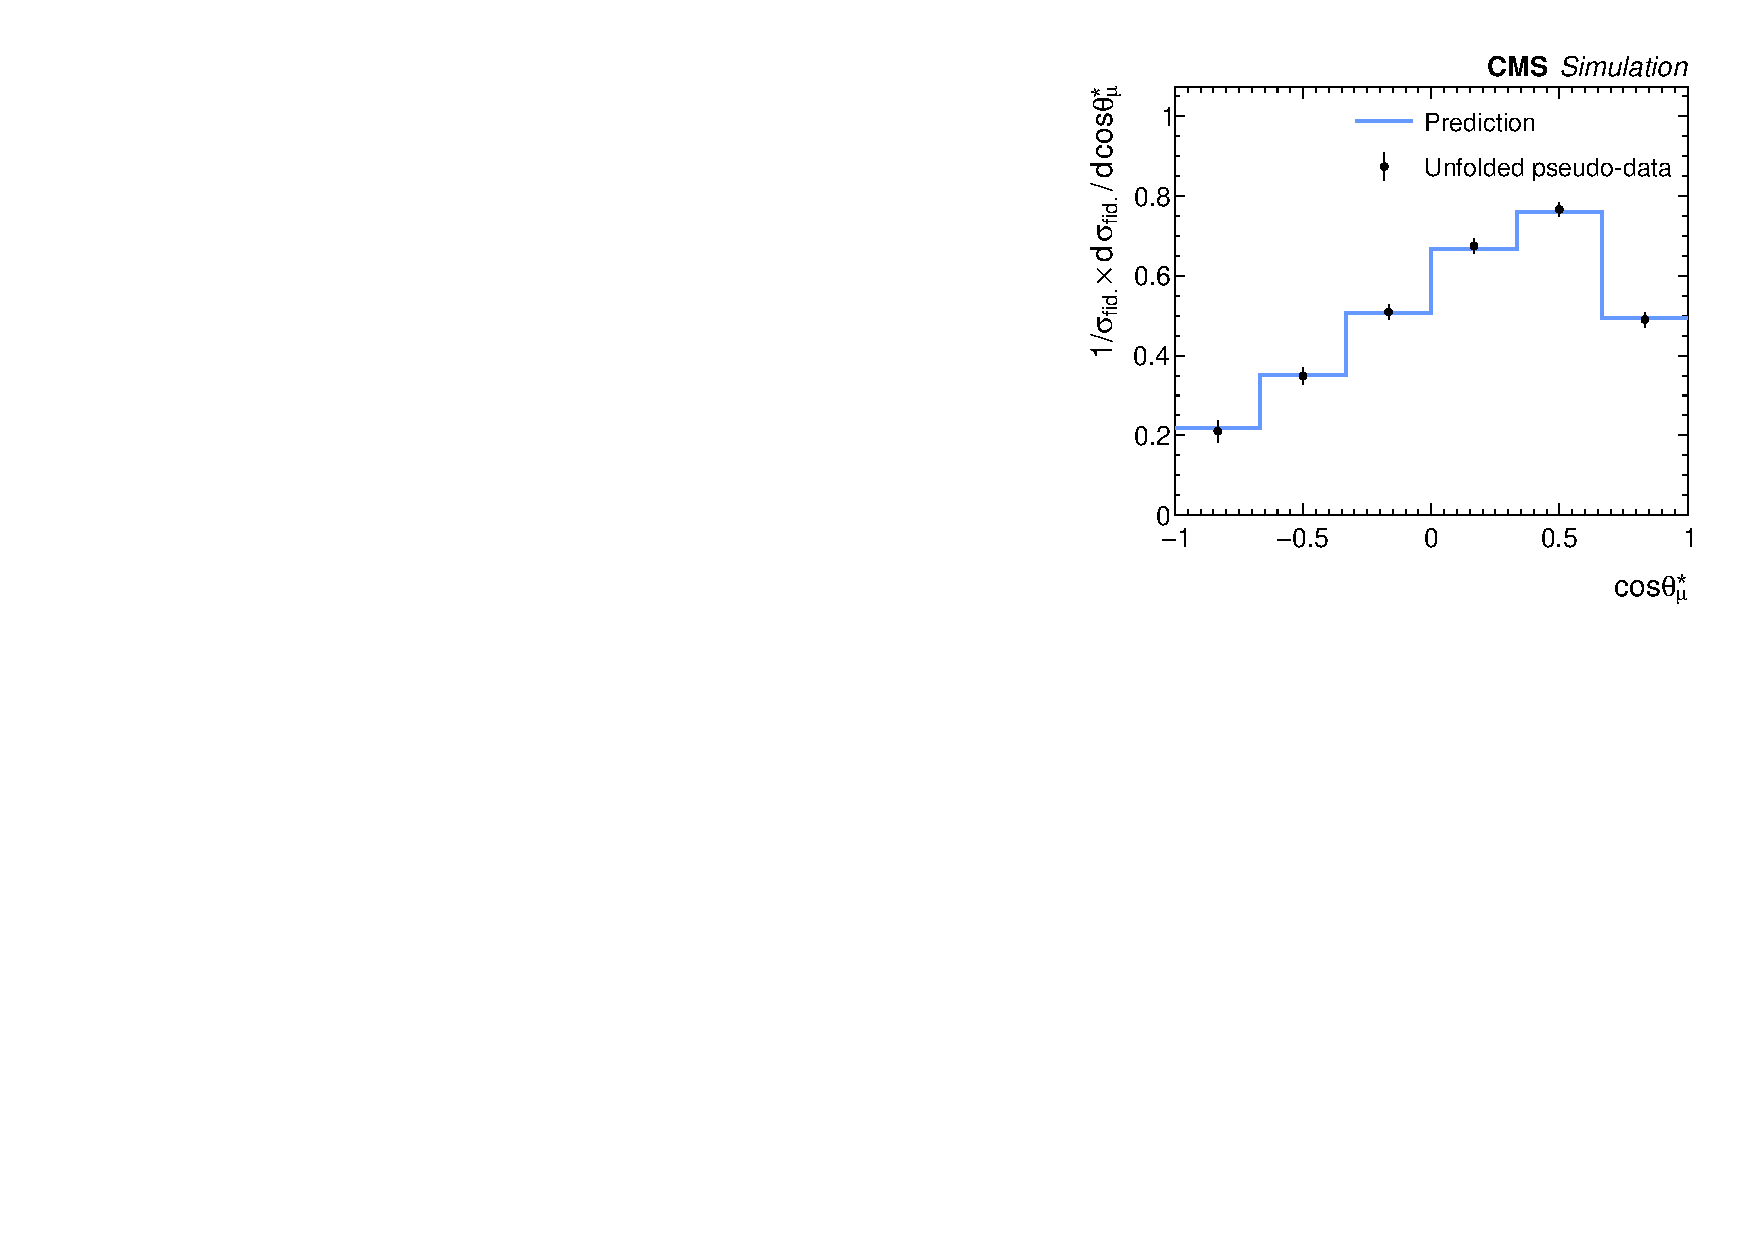
\includegraphics[width=0.48\textwidth]{figures/prospects/unfolding/unfoldedParticle_mu_cos.pdf}}\hspace{0.02\textwidth}
\subfloat[]{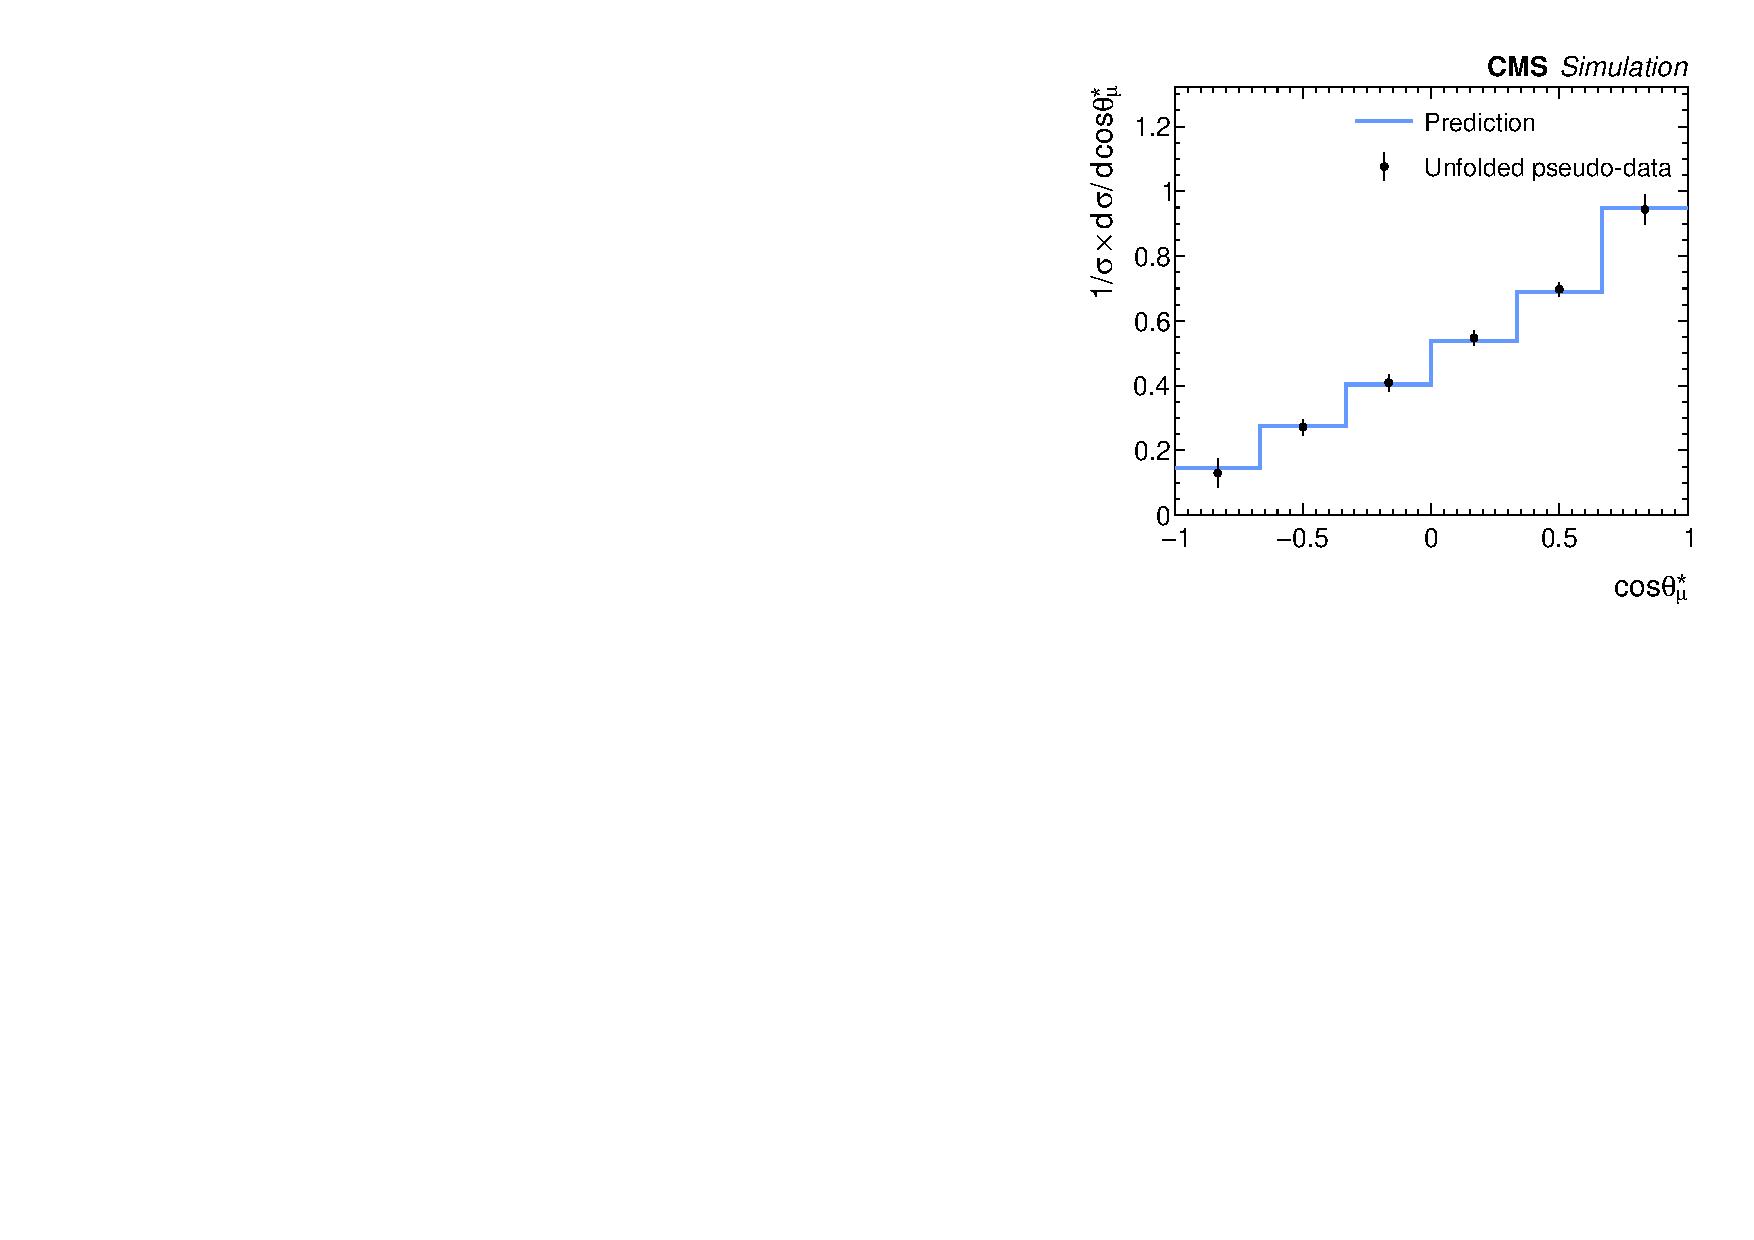
\includegraphics[width=0.48\textwidth]{figures/prospects/unfolding/unfoldedParton_mu_cos.pdf}}
}

